\section{Parallel and generalised NOAH supersequences}
\label{sec:noah__parallel}

To conclude this chapter, I discuss how \textit{multiple} NOAH supersequences may be run in parallel in order to obtain yet more data from a single experiment.
As of the time of writing, current software limitations in TopSpin limit the \texttt{NBL} parameter (the number of memory blocks) to 5.
This makes it presently impossible to extend a supersequence linearly beyond five modules.
However, it is possible to \textit{interleave} different supersequences, such that one $t_1$ increment of supersequence A is acquired, followed by one $t_1$ increment of supersequence B, before the value of $t_1$ is increased for both supersequences.
In this text, I refer to this as a `vertical' stacking of modules (as opposed to the traditional NOAH concept, which focuses on `horizontal' concatenation of modules).

\subsection{Parallel NOAH supersequences}
\label{sec:noah__parallel_parallel}

\begin{figure}[!htbp]
    \centering
    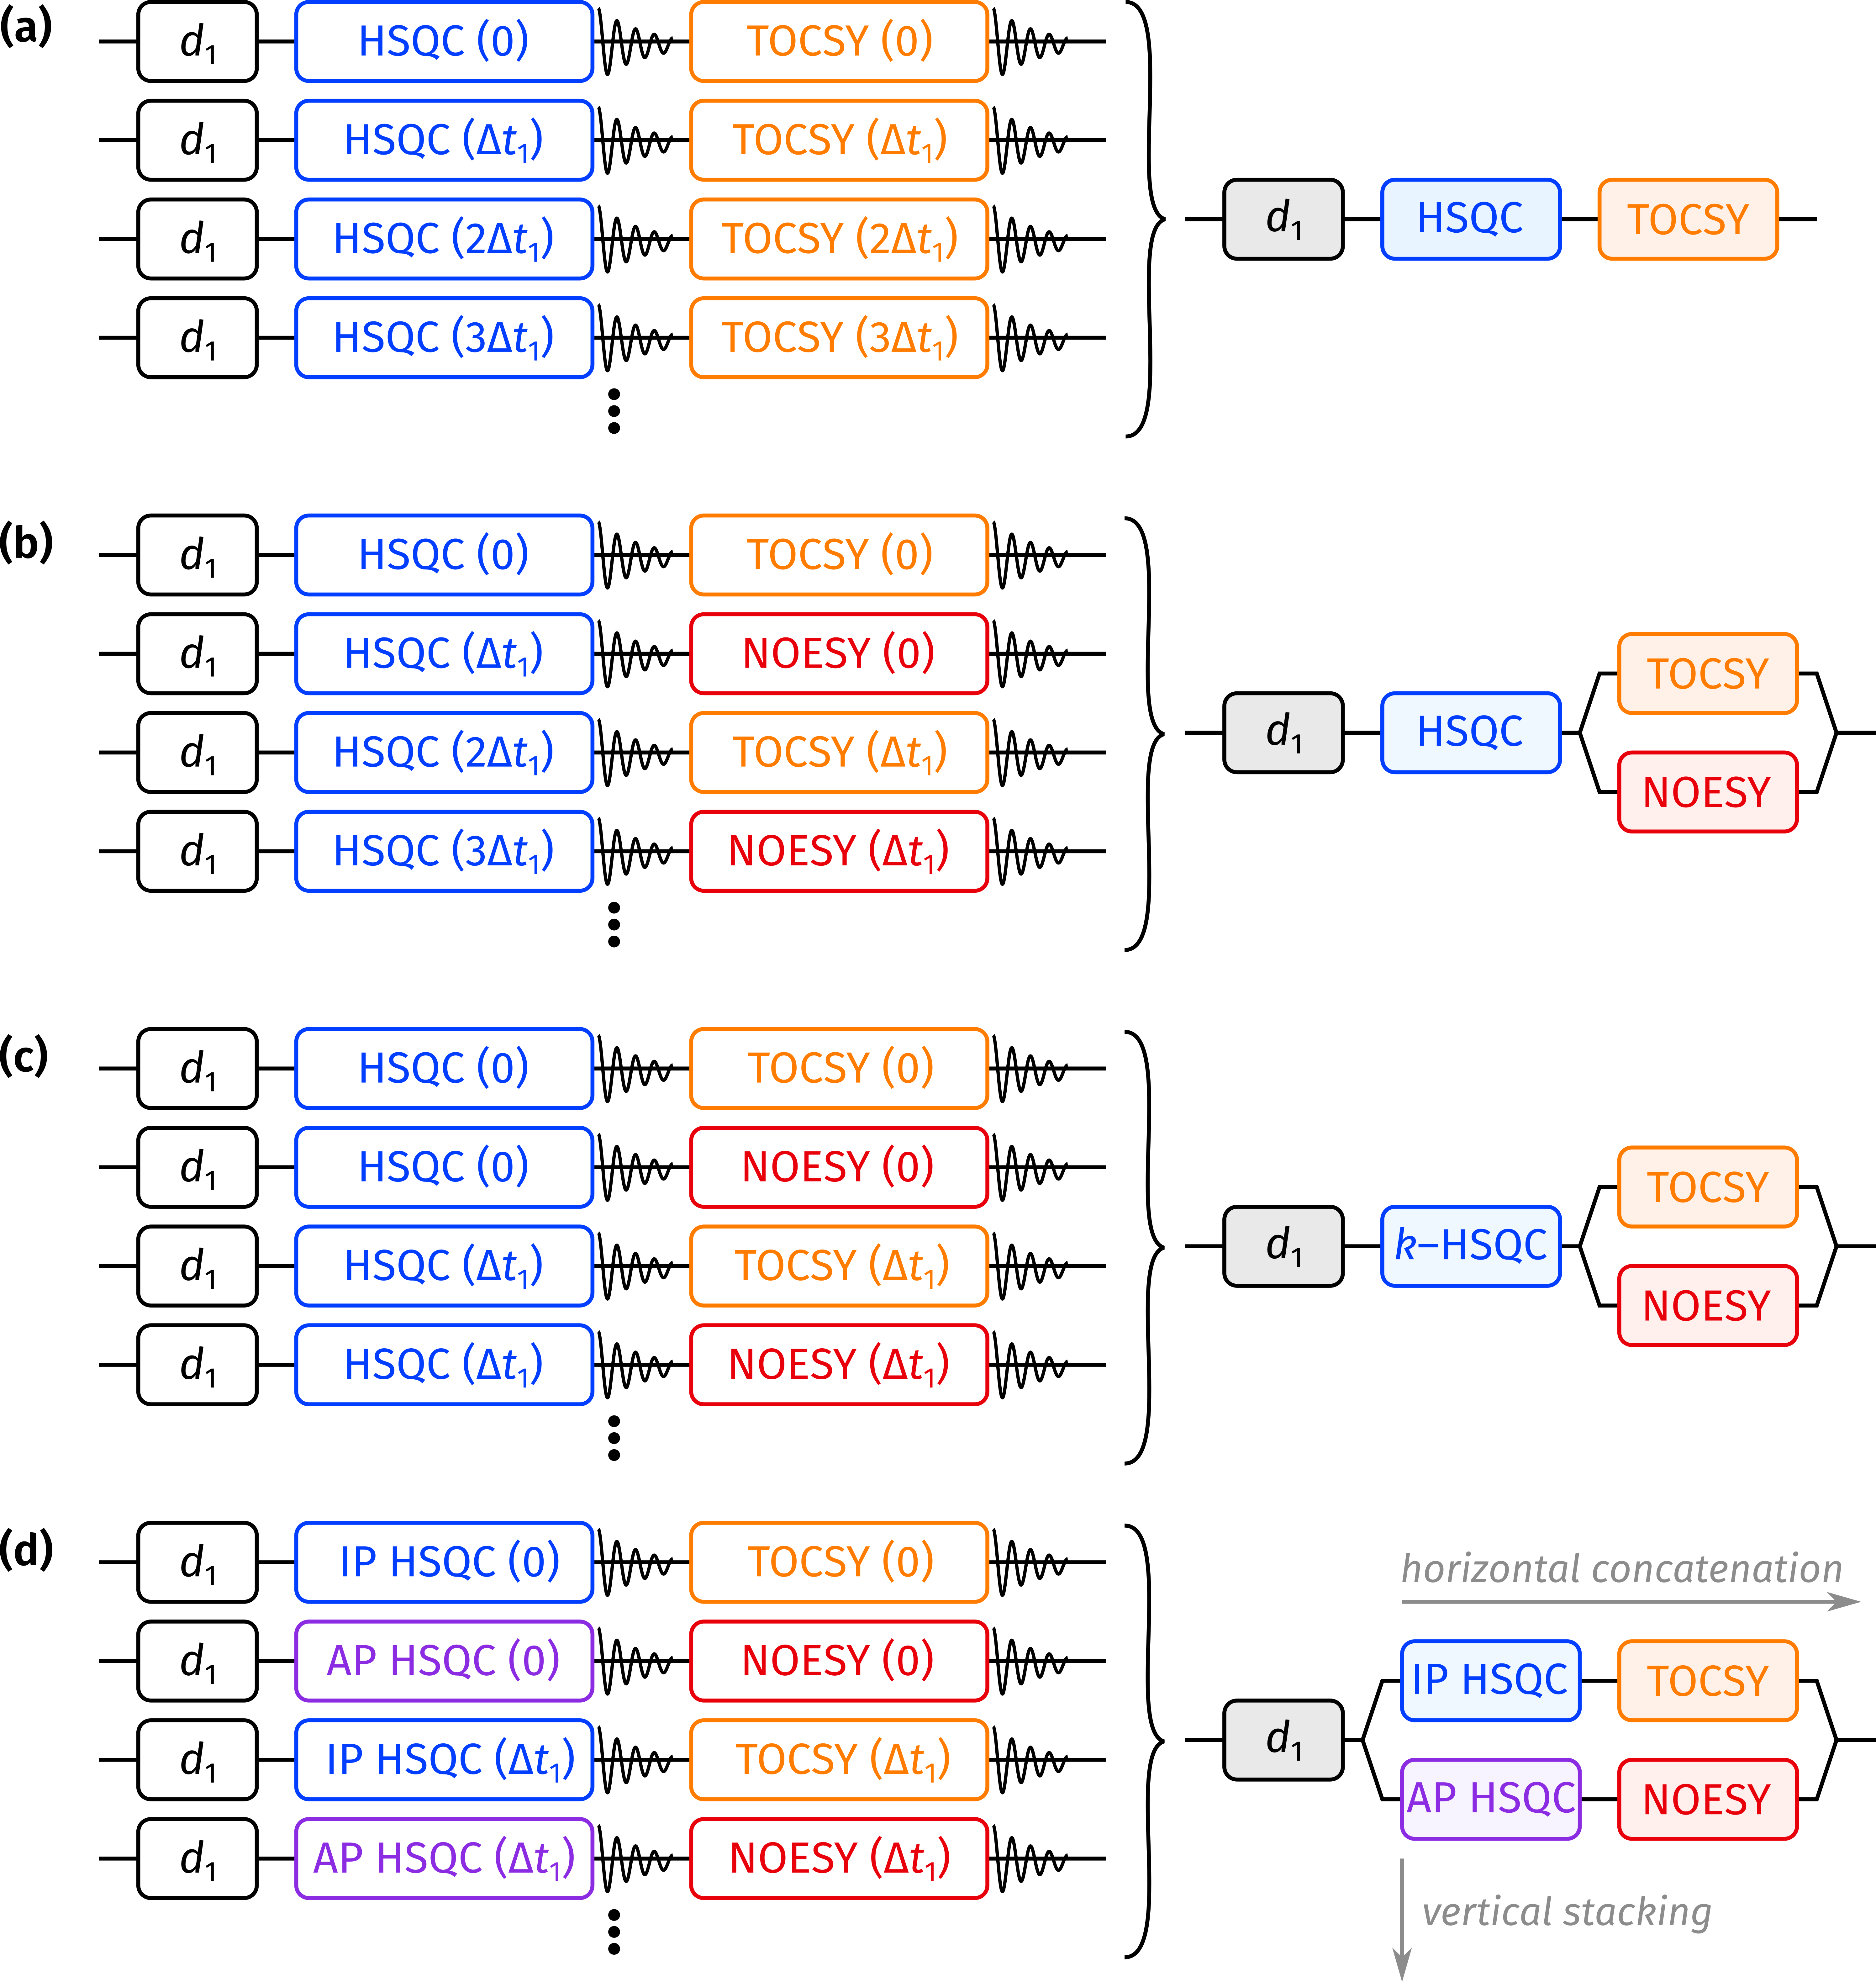
\includegraphics[draft=false]{noah/parallel_noah_overview.png}%
    {\phantomsubcaption\label{fig:parallel_noah_overview_conv}}%
    {\phantomsubcaption\label{fig:parallel_noah_overview_interleaved}}%
    {\phantomsubcaption\label{fig:parallel_noah_overview_kscaled}}%
    {\phantomsubcaption\label{fig:parallel_noah_overview_parallel}}%
    \caption[Overview of parallel NOAH supersequences]{
        An overview of `parallel' NOAH supersequences.
        The left side of each diagram explicitly spells out how $t_1$ is incremented for each module: the value in parentheses indicates the current value of $t_1$, which begins at 0 and is incremented by $\Delta t_1$ each time.
        The right side is a `condensed' depiction of the entire supersequence.
        \textbf{(\subref*{fig:parallel_noah_overview_conv})} A `standard' NOAH supersequence, where $t_1$ for every module is incremented at the same time.
        \textbf{(\subref*{fig:parallel_noah_overview_interleaved})} The first example of a `parallel' supersequence: the HSQC module is acquired as normal, but the TOCSY and NOESY modules are interleaved in the second slot.
        \textbf{(\subref*{fig:parallel_noah_overview_kscaled})} The same as in (\subref*{fig:parallel_noah_overview_interleaved}), but the HSQC module is subjected to $k$-scaling (see also \cref{subsec:noah__hmqc}).
        \textbf{(\subref*{fig:parallel_noah_overview_parallel})} A fully parallel supersequence, where both the first and second module slots are varied systematically.
        This amounts to the interleaved acquisition of two different `standard' supersequences.
    }
    \label{fig:parallel_noah_overview}
\end{figure}

This concept is more clearly illustrated in \cref{fig:parallel_noah_overview}, which contains a more explicit depiction of how $t_1$ is incremented for each module.
In \cref{fig:parallel_noah_overview_conv}, a `traditional' \noah{S,T} supersequence is shown: here, $t_1$ is incremented for both the HSQC and TOCSY module at the same time, and on each $t_1$ increment, the sequence of modules being acquired is always the same.
In \cref{fig:parallel_noah_overview_interleaved}, this is different: the second module is alternated between a TOCSY and a NOESY.
If the total experimental duration (which is largely proportional to the number of recovery delays, $d_1$) is to be kept the same as before, this means that the TOCSY and NOESY modules will be recorded with half the number of $t_1$ increments each.%
\footnote{The data must also be separated prior to Fourier transformation in the indirect dimension. This is `just' an implementation detail, but \textit{did} require the \texttt{splitx\_au} script to be substantially reworked.}
Although this loss of resolution may be considered a drawback, this scheme does allow us greater \textit{flexibility} in the design of NOAH supersequences: it is not ideal to acquire both a TOCSY and a NOESY using a traditional `linear' supersequence, since both of these modules depend on \magnnot{C} magnetisation.

\Cref{fig:parallel_noah_overview_kscaled} shows how the different $F_1$ resolutions can be `fixed' by performing the equivalent of $k$-scaling on the HSQC module (described in \cref{subsec:noah__hmqc}).
This entails reducing the number of $t_1$ increments by a factor of 2 (in this case), and acquiring each increment twice instead, which corresponds to a doubling of the number of scans after the data have been appropriately combined.
This generally has very little impact on the spectra (as was previously shown), but provides a convenient lead into the final example of \cref{fig:parallel_noah_overview_parallel}.
Here, instead of acquiring each increment of the HSQC module twice, the time is used to acquire two different modules, an in-phase (IP) and antiphase (AP) HSQC (both run without \carbon{} decoupling).
Through appropriate linear combination of the data, it is possible to isolate the two peaks of the \proton{}--\carbon{} doublets in these spectra, and from thence measure $\oneJ{CH}$ values: this is known as in-phase/antiphase (IPAP) processing.\autocite{Ottiger1998JMR,Nolis2006JMR,Enthart2008JMR,Gil2010JMR}
Much like the TOCSY and NOESY combination, it is not possible to acquire IP and AP HSQC spectra in a single, linear supersequence, not even with the partial \magn{C} excitation technique described in \cref{subsec:noah__hsqctocsy}.
For the IPAP processing to work, the IP and AP spectra have to be acquired with the same intensity for all peaks: even with a careful choice of $f$ in a linear supersequence, it is not possible to ensure this.

The reader will no doubt notice at this point that \cref{fig:parallel_noah_overview_parallel} corresponds simply to the interleaved acquisition of two different supersequences (one is IP-HSQC + COSY, and the other AP-HSQC + NOESY), which could just as well be acquired separately.
Furthermore, both supersequences are acquired with only half the usual $F_1$ resolution (assuming the same experimental time as \cref{fig:parallel_noah_overview_conv}), meaning that there are \textit{no real time savings}.
This is indeed correct: fundamentally, `vertical' stacking does not increase the number of FIDs recorded per recovery delay, so does not improve the time efficiency (or $\rho_t$).
The main benefits of this process are, in my opinion:
\begin{itemize}
    \item the \textit{flexibility} to construct supersequences that combine previously incompatible modules (such as in the examples above); and
    \item a way of \textit{adjusting for relative sensitivities of different modules}.
        For example, the arrangement in \cref{fig:parallel_noah_overview_kscaled} amounts to the acquisition of the HSQC module for $2n$ scans, and the TOCSY and NOESY modules for $n$ scans each (where $n$ is some positive integer).
        In this way, less intrinsically sensitive modules can be assigned a larger number of scans, such that all modules in the supersequence have (relatively) equalised intensities.
\end{itemize}

In principle, all of the above may still be accomplished in a roundabout manner by acquiring multiple separate supersequences and then combining the results.
This is most obvious in \cref{fig:parallel_noah_overview_parallel}.
However, the current implementation of parallel supersequences provides \textit{convenience} for the user, as all experiments may be simultaneously acquired and processed.
This factor should not be overlooked, especially considering that all the different constructions (\cref{fig:parallel_noah_overview_interleaved,fig:parallel_noah_overview_kscaled,fig:parallel_noah_overview_parallel}) must be processed in a slightly different manner: it is easier to do this from within a single experiment, rather than attempting to combine FIDs from separate datasets after the fact.
There is also another argument for acquiring increments in an interleaved manner: this helps to minimise drifts in the spectra which arise from temporal instabilities in (for example) temperature.

\begin{figure}[!ht]
    \centering
    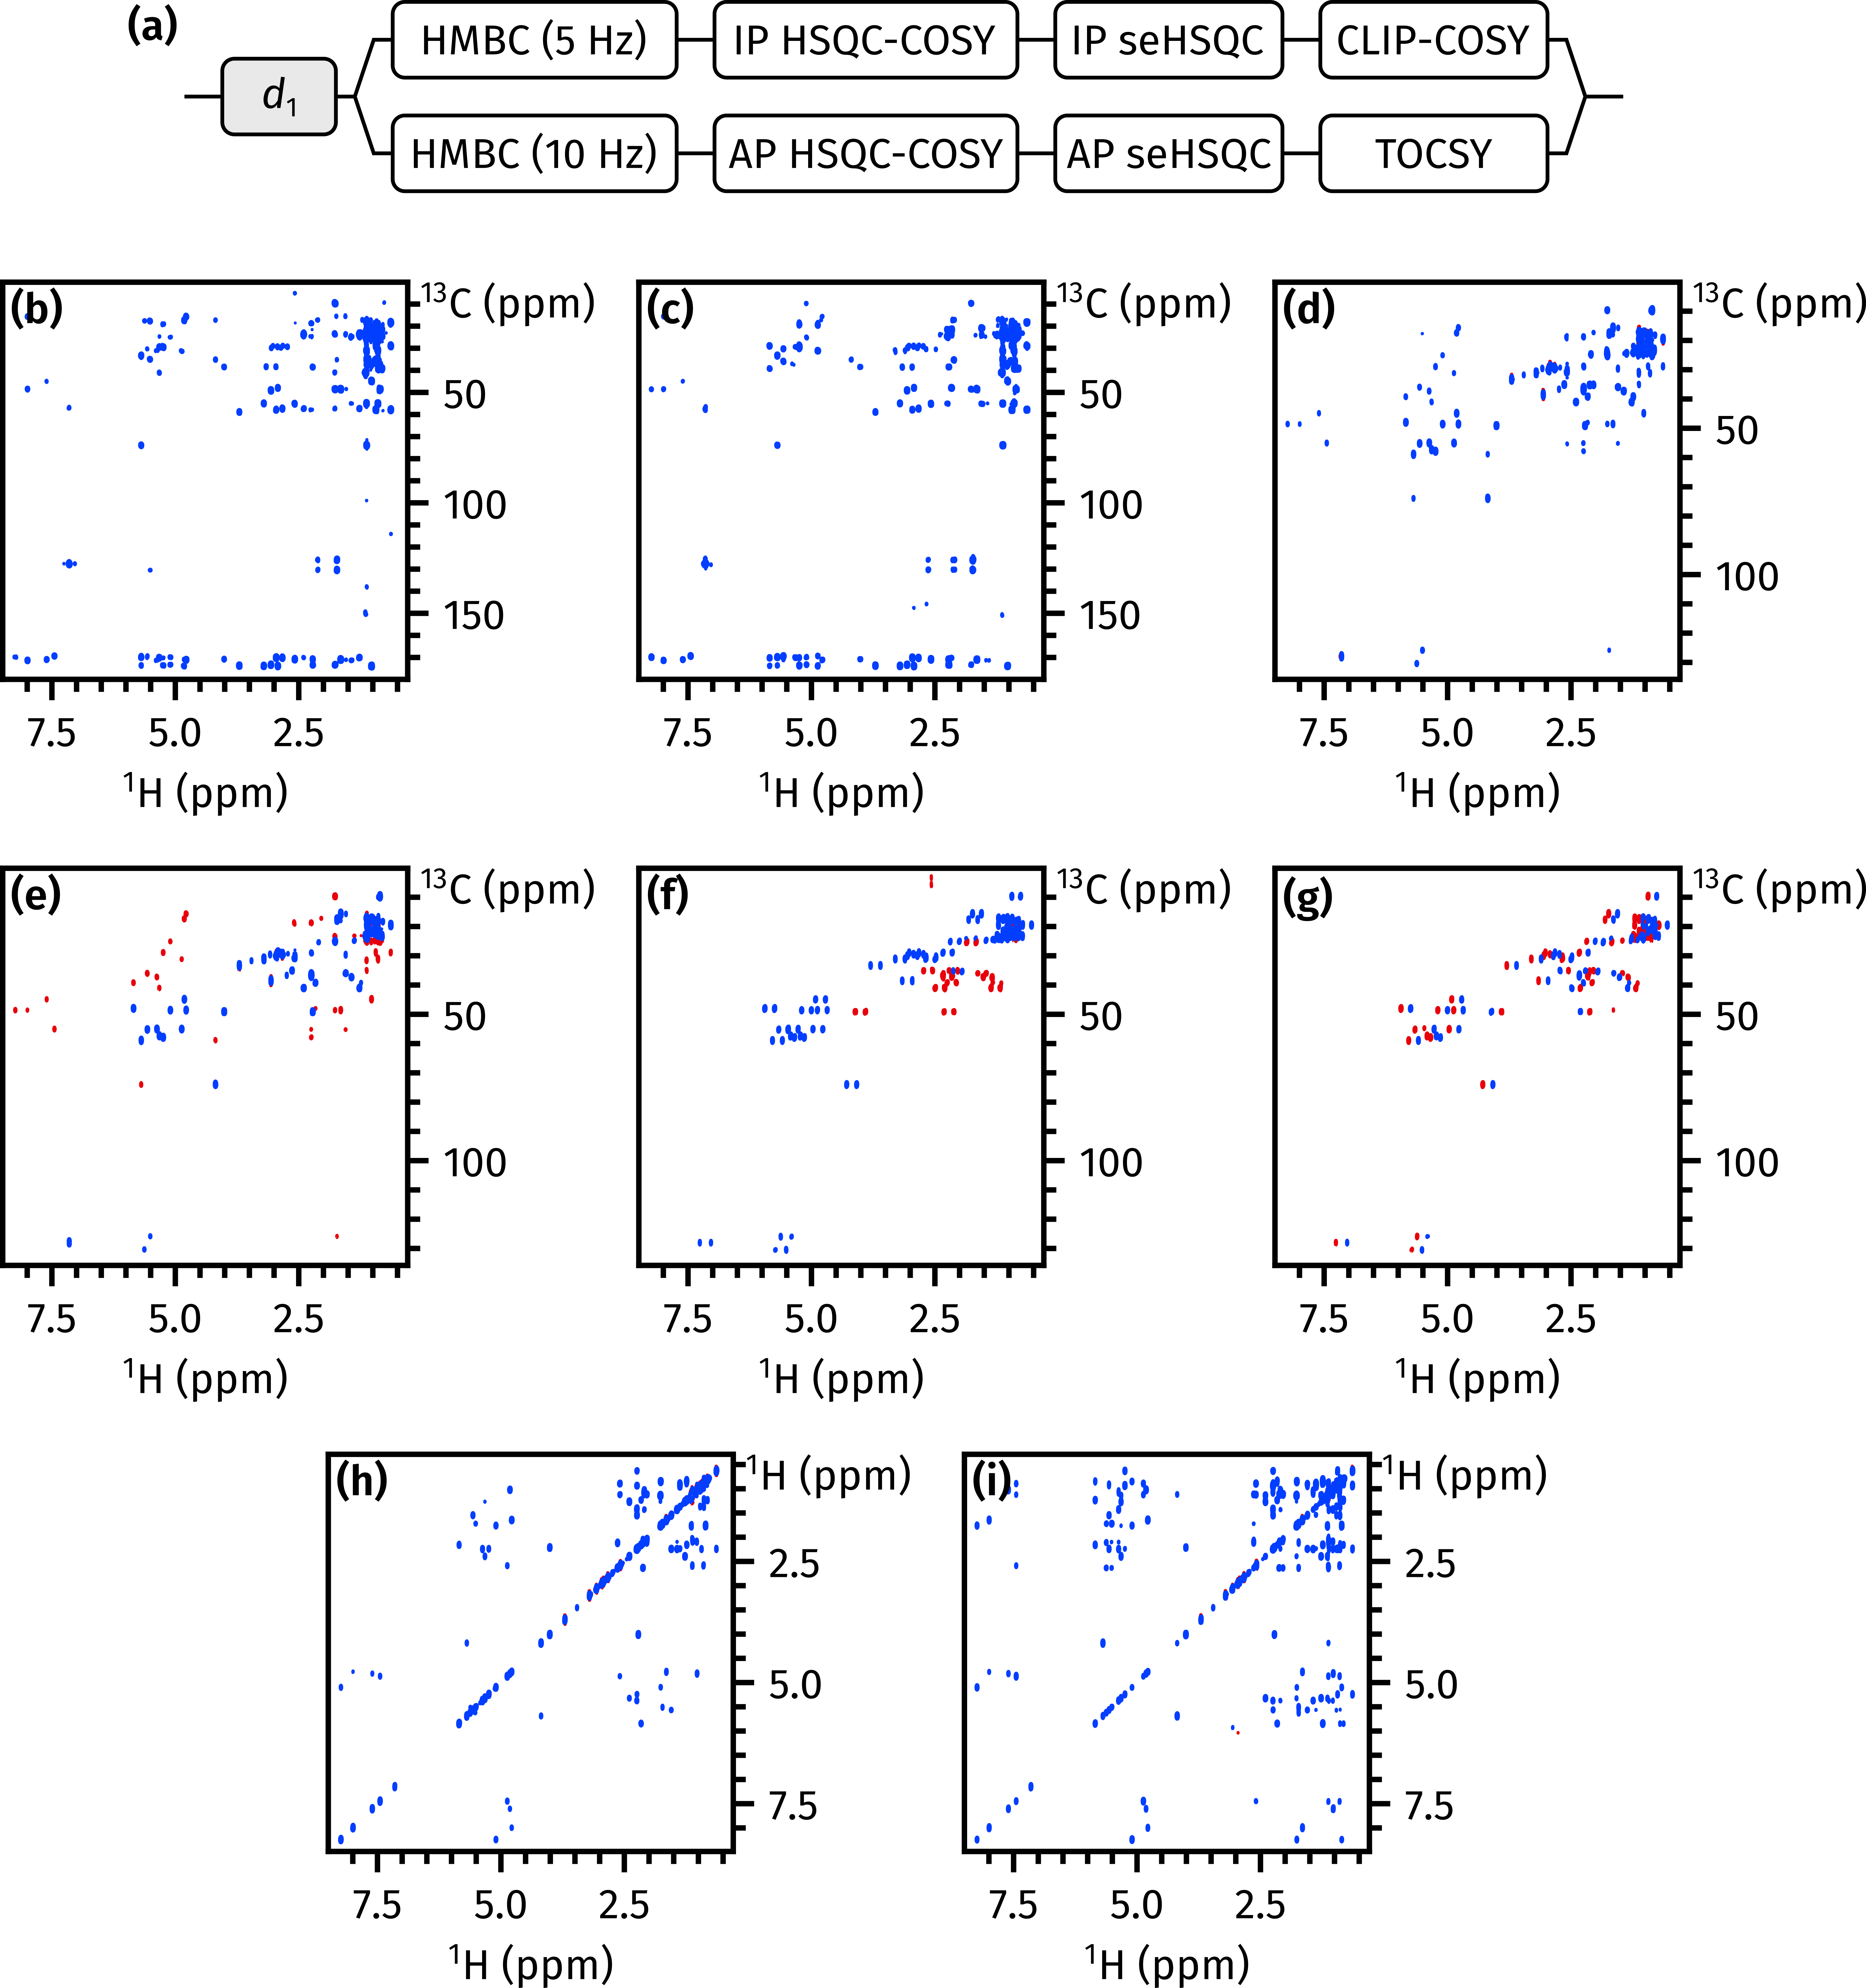
\includegraphics[draft=false]{noah/tsnoah_example.png}%
    {\phantomsubcaption\label{fig:tsnoah_example_overall}}%
    {\phantomsubcaption\label{fig:tsnoah_example_b1}}%
    {\phantomsubcaption\label{fig:tsnoah_example_b2}}%
    {\phantomsubcaption\label{fig:tsnoah_example_sc1}}%
    {\phantomsubcaption\label{fig:tsnoah_example_sc2}}%
    {\phantomsubcaption\label{fig:tsnoah_example_s1}}%
    {\phantomsubcaption\label{fig:tsnoah_example_s2}}%
    {\phantomsubcaption\label{fig:tsnoah_example_cc}}%
    {\phantomsubcaption\label{fig:tsnoah_example_t}}%
    \caption[Spectra from a NOAH-8 `parallel' supersequence]{
        \textbf{(\subref*{fig:tsnoah_example_overall})} Condensed representation of the supersequence, which may be interpreted in the same way as \cref{fig:parallel_noah_overview_parallel}.
        \textbf{(\subref*{fig:tsnoah_example_b1})} HMBC, optimised for $\nJ{CH} = \qty{5}{\Hz}$.
        \textbf{(\subref*{fig:tsnoah_example_b2})} HMBC, optimised for $\nJ{CH} = \qty{10}{\Hz}$.
        \textbf{(\subref*{fig:tsnoah_example_sc1})} IP HSQC-CLIP-COSY.
        \textbf{(\subref*{fig:tsnoah_example_sc2})} AP HSQC-CLIP-COSY.
        \textbf{(\subref*{fig:tsnoah_example_s2})} IP multiplicity-edited seHSQC.
        \textbf{(\subref*{fig:tsnoah_example_s2})} AP multiplicity-edited seHSQC.
        \textbf{(\subref*{fig:tsnoah_example_cc})} CLIP-COSY.
        \textbf{(\subref*{fig:tsnoah_example_t})} TOCSY (\qty{60}{\ms} mixing time).
    }
    \label{fig:tsnoah_example}
\end{figure}

\Cref{fig:tsnoah_example_overall} shows one example of a more complex parallel supersequence containing 8 modules.
In this supersequence, the HMBC module is recorded twice with the delay $\Delta_\text{LR}$ optimised for two different values of $\nJ{CH}$ (\cref{fig:tsnoah_example_b1,fig:tsnoah_example_b2}): these spectra furnish a (slightly) different set of correlations, which allow for more complete structure determination.
The HSQC-CLIP-COSY is acquired in an IPAP fashion, where direct/indirect editing is used in one experiment (\cref{fig:tsnoah_example_sc2}) and not in the other (\cref{fig:tsnoah_example_sc1}).
Likewise, the $F2$-coupled seHSQC experiment is also performed in an IPAP manner, where this time the `IPAP' components are the two peaks in each doublet.
Multiplicity editing is additionally used here in both IP and AP seHSQC spectra.
Finally, we have two interleaved homonuclear modules, the CLIP-COSY and TOCSY (\cref{fig:tsnoah_example_cc,fig:tsnoah_example_t}), which provide complementary information about spin networks.
The four IPAP-processed spectra from this supersequence are shown in \cref{fig:tsnoah_ipap_spec}.

\begin{figure}[!ht]
    \centering
    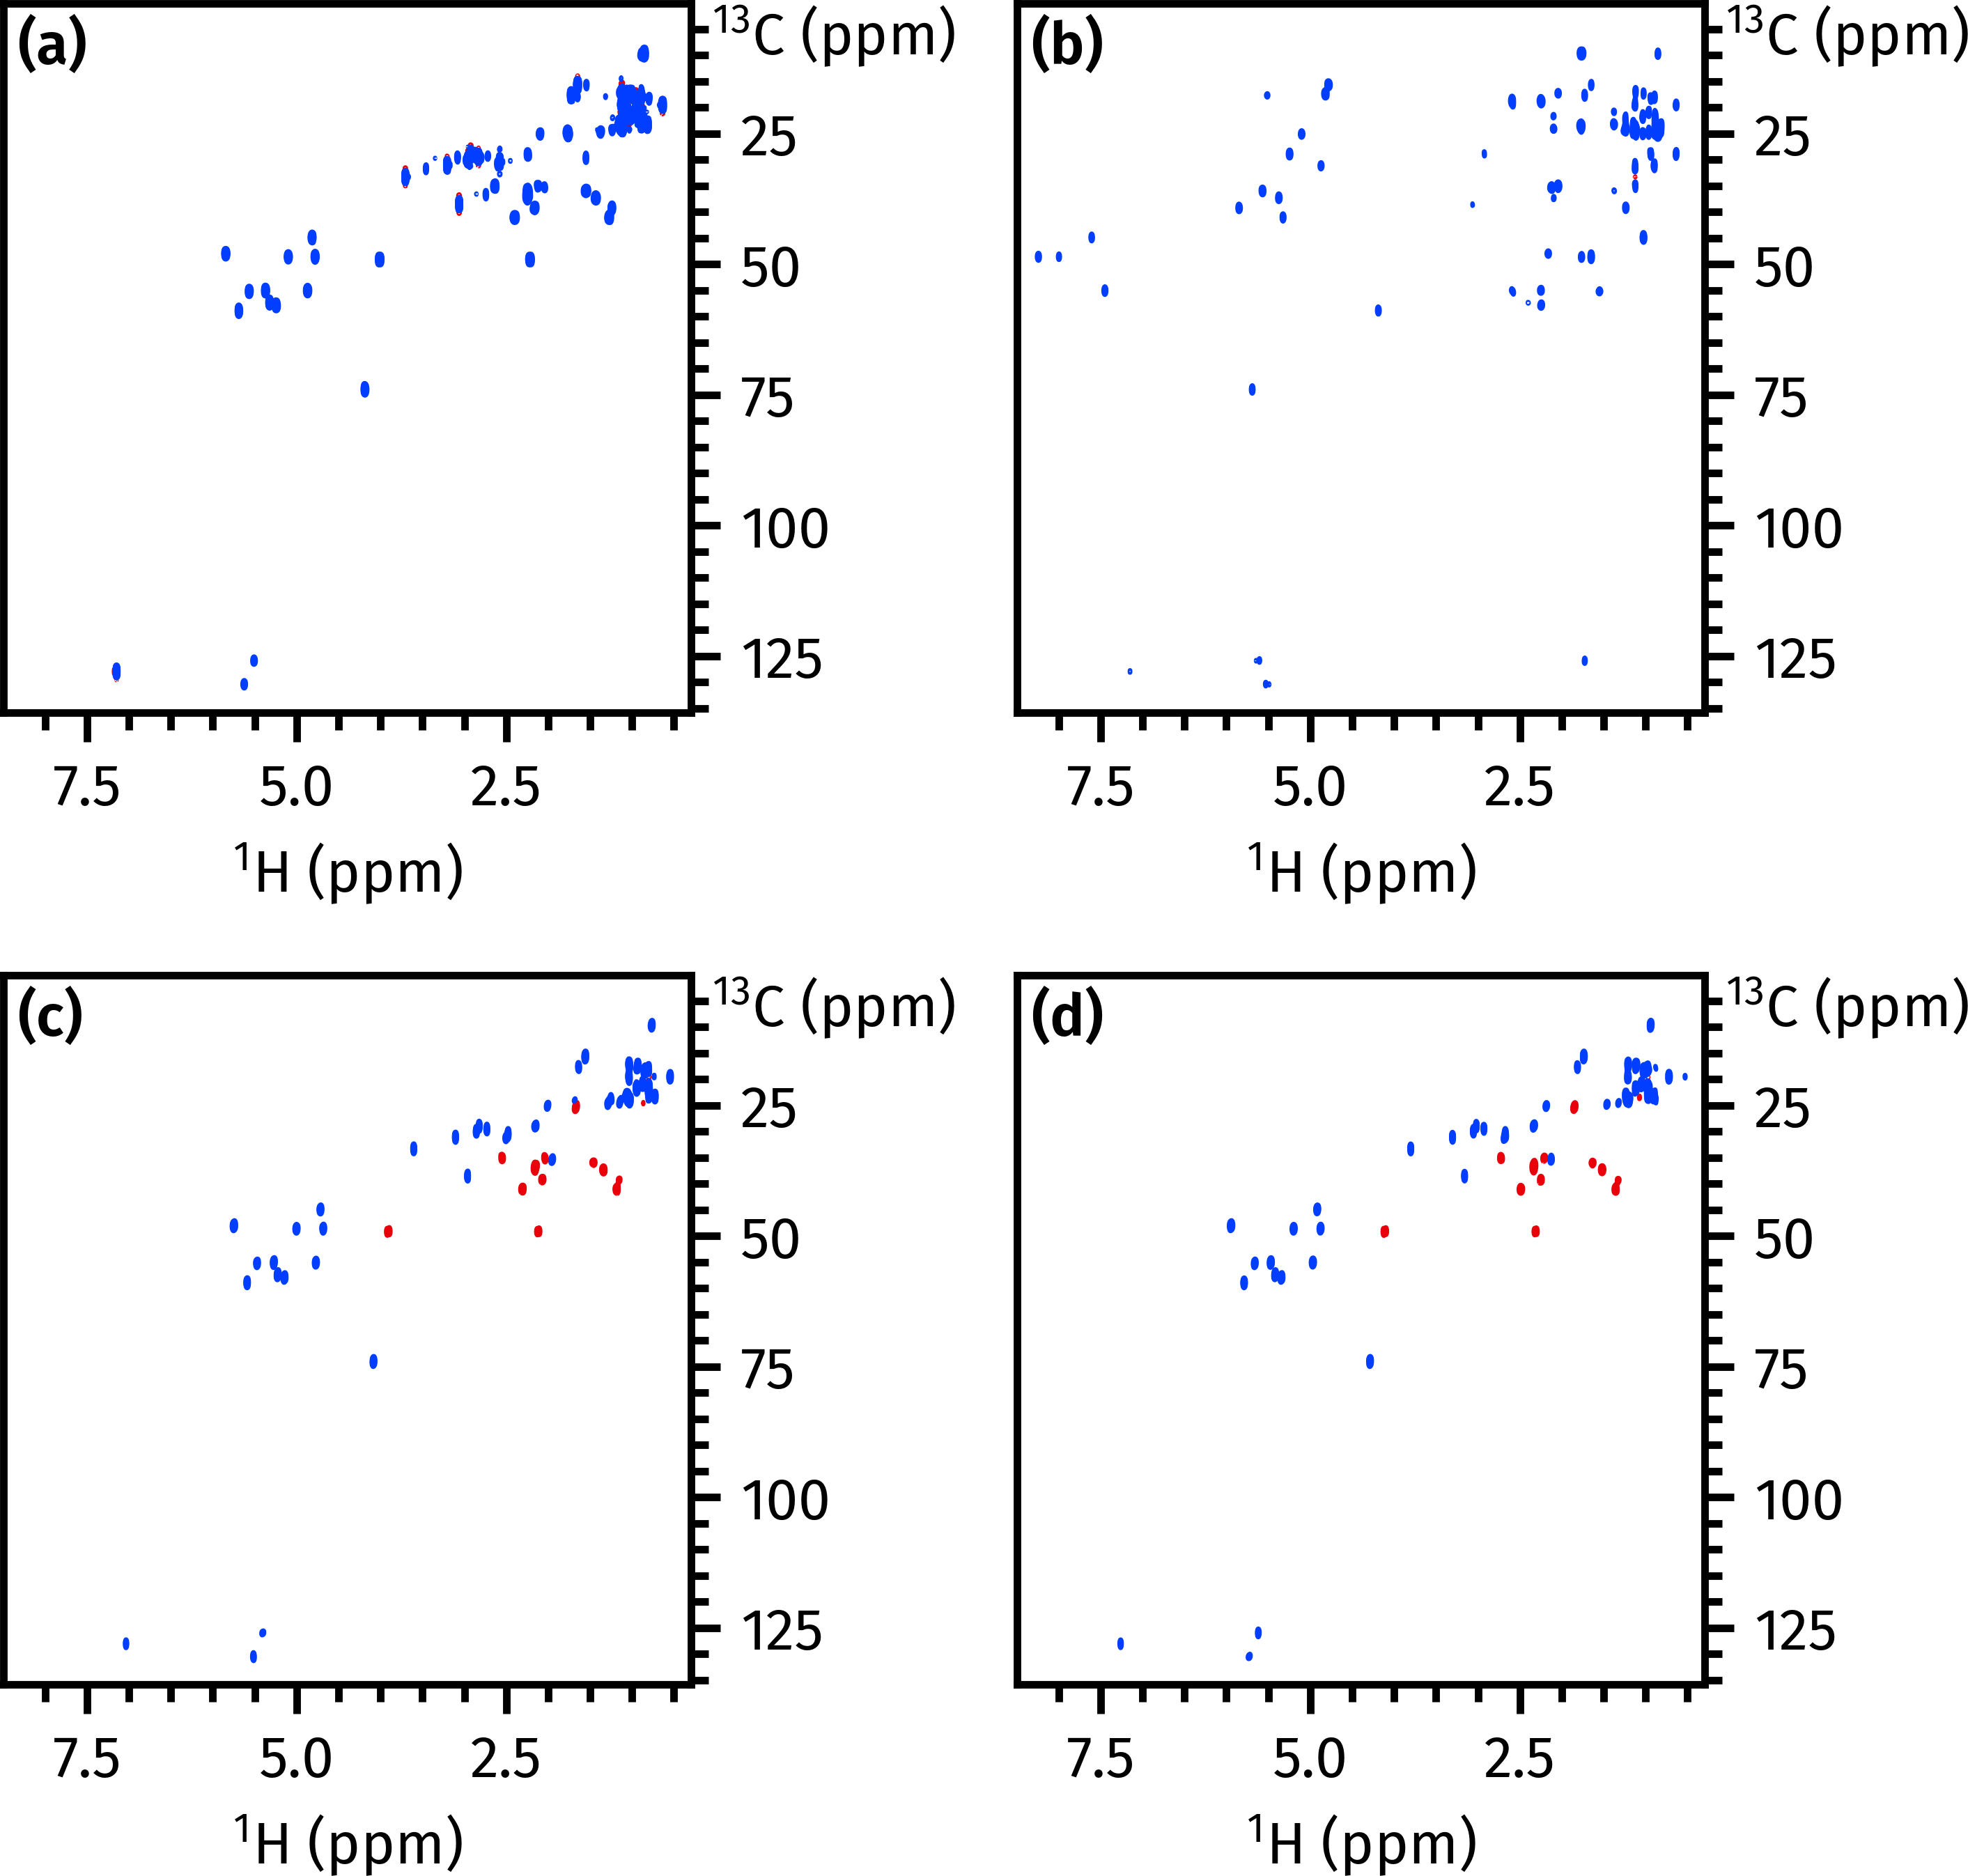
\includegraphics[draft=false]{noah/tsnoah_ipap_spec.png}%
    {\phantomsubcaption\label{fig:tsnoah_ipap_spec_sc_direct}}%
    {\phantomsubcaption\label{fig:tsnoah_ipap_spec_sc_indirect}}%
    {\phantomsubcaption\label{fig:tsnoah_ipap_spec_s_alpha}}%
    {\phantomsubcaption\label{fig:tsnoah_ipap_spec_s_beta}}%
    \caption[IPAP processed spectra from NOAH-8 supersequence]{
        \textbf{(\subref*{fig:tsnoah_ipap_spec_sc_direct})--(\subref*{fig:tsnoah_ipap_spec_sc_indirect})} IPAP-processed HSQC-COSY spectra (from \cref{fig:tsnoah_example_sc1,fig:tsnoah_example_sc2}), which separate the `direct' and `indirect' HSQC-COSY responses described in \cref{subsec:noah__hsqccosy}.
        \textbf{(\subref*{fig:tsnoah_ipap_spec_s_alpha})--(\subref*{fig:tsnoah_ipap_spec_s_beta})} IPAP-processed seHSQC spectra (from \cref{fig:tsnoah_example_s1,fig:tsnoah_example_s2}), each of which contain one peak of each \proton{}--\carbon{} doublet.
    }
    \label{fig:tsnoah_ipap_spec}
\end{figure}

\subsubsection{Time-shared NMR}

In my published work\autocite{Kupce2021JACSA}, what I refer to as IPAP here is frequently labelled as a TS, or \textit{time-shared} experiment.
In TS NMR, pulse sequences are specially designed in order to record two (or more) different signals at once, such as a \carbon{} HSQC and a \nitrogen{} HSQC: this has found use in both biomolecular\autocite{Farmer1991JMR,Boelens1994JBNMR,Pascal1994JMRSB,Sattler1995JBNMR,Frueh2009JBNMR,Lohr2014JMR} and small-molecule NMR\autocite{Nolis2006MRC,PerezTrujillo2007OL,Nolis2007ACIE,Parella2010CMR}.
Often, the design of TS experiments involves the joint evolution of both heteronuclear chemical shifts in a shared $t_1$ period: hence the term `time-shared'.

It should be noted that TS experiments use \textit{simultaneous} acquisition, as opposed to the \textit{sequential} acquisition of NOAH experiments.
In other words, the two or more signals recorded in a TS experiment are part of the same FID, meaning that the resulting spectra will contain peaks from both signals.
If these can be easily disambiguated (e.g.\ by the differing chemical shifts of \carbon{}- or \nitrogen{}-bonded protons), then the TS experiment allows more data to be collected in the same amount of time as a non-TS experiment.
However, if these signals must be separated, then the TS experiment must be repeated: once where the two signals have the same phase, and once where they have opposite phases.
The underlying signals can then be disentangled through linear combination.\autocite{Sorensen1990JMR,Farmer1991JMR}

Mathematically, this is exactly the same process as IPAP processing.
In my view, what separates the two is the fact that the IPAP technique seeks to disentangle components which are \textit{innate} to the pulse sequence under consideration and cannot usually be isolated---such as doublets in a $F_2$-coupled HSQC---whereas TS experiments must be \textit{specially crafted} to record these multiple components.
Equivalently, the time savings (or sensitivity improvement) from a TS experiment stem from the fact that it is being compared against a pair of experiments which each yield only one of the two signals detected in the TS sequence.

In this case, the IPAP label clearly applies to the pair of $F_2$-coupled seHSQC modules in \cref{fig:tsnoah_example_s1,fig:tsnoah_example_s2}.
However, for the HSQC-COSY modules in \cref{fig:tsnoah_example_sc1,fig:tsnoah_example_sc2}, the situation is less clear.
The two `signals' which we should consider are the `direct' and `indirect' peaks; however, it is not entirely obvious which experiments can be used for these.
The `direct' peaks correspond to a (\carbon{}-decoupled) HSQC experiment.%
\footnote{It should be noted that the intensities of the direct peaks in an HSQC-COSY spectrum are lower than in the corresponding HSQC spectrum, because the direct peaks in an HSQC-COSY stem only from magnetisation which does \textit{not} evolve under $\nJ{HH}$ during the mixing period. However, TS experiments do generally have lower sensitivity than the non-TS counterparts, so this is not really an issue.}
However, for the `indirect' peaks, there is no real equivalent spectrum to be compared against: the H2BC experiment\autocite{Nyberg2005JACS,Nyberg2005MRC} yields a similar set of peaks, but in this experiment, the `direct' peaks have in fact been intentionally suppressed through the application of a LPJF.
When the LPJF is removed (as in the 2BOB/H2OBC experiments\autocite{Kupce2017MRC}), a similar information content to the HSQC-COSY is obtained.
So, it is not entirely accurate to write that the HSQC-COSY combines a HSQC plus H2BC spectrum.
Consequently, I personally prefer to view it as an IPAP experiment.

Of course, the analysis above is only applicable to the modules shown in \cref{fig:tsnoah_example}.
None of this precludes the application of \textit{true} time-shared experiments to NOAH supersequences: it is completely possible to implement, for example, a \carbon{}/\nitrogen{} TS experiment within the context of a parallel supersequence.
However, many TS experiments are already designed to detect signals arising from different magnetisation pools (e.g.\ \magn{C} and \magn{N}).
This is already something which can be accomplished in a cleaner manner using (linear) NOAH supersequences.



\subsection{Generalised supersequences}
\label{sec:noah__parallel_generalised}

From the discussion above, it is evident that there is no need to stop at \textit{two} interleaved modules: it is possible to endlessly stack modules in a vertical manner.
Furthermore, different modules may be acquired a different number of times.
Thus, in \cref{fig:parallel_noah_overview_interleaved}, two supersequences were interleaved, and the TOCSY and NOESY modules were acquired once each in each $t_1$ increment.
However, if $M$ different supersequences are being interleaved, then a set of two different modules may be acquired $m_1$ and $m_2$ times, as long as $m_1 + m_2 = M$.
For example, a supersequence with $m_1 = 1$ and $m_2 = 3$ is shown in \cref{fig:generalised_example}.
Generally, it is desirable to assign larger $m_i$ values to less sensitive modules, as the results can be summed up to yield improved signal-to-noise.

\begin{figure}[!ht]
    \centering
    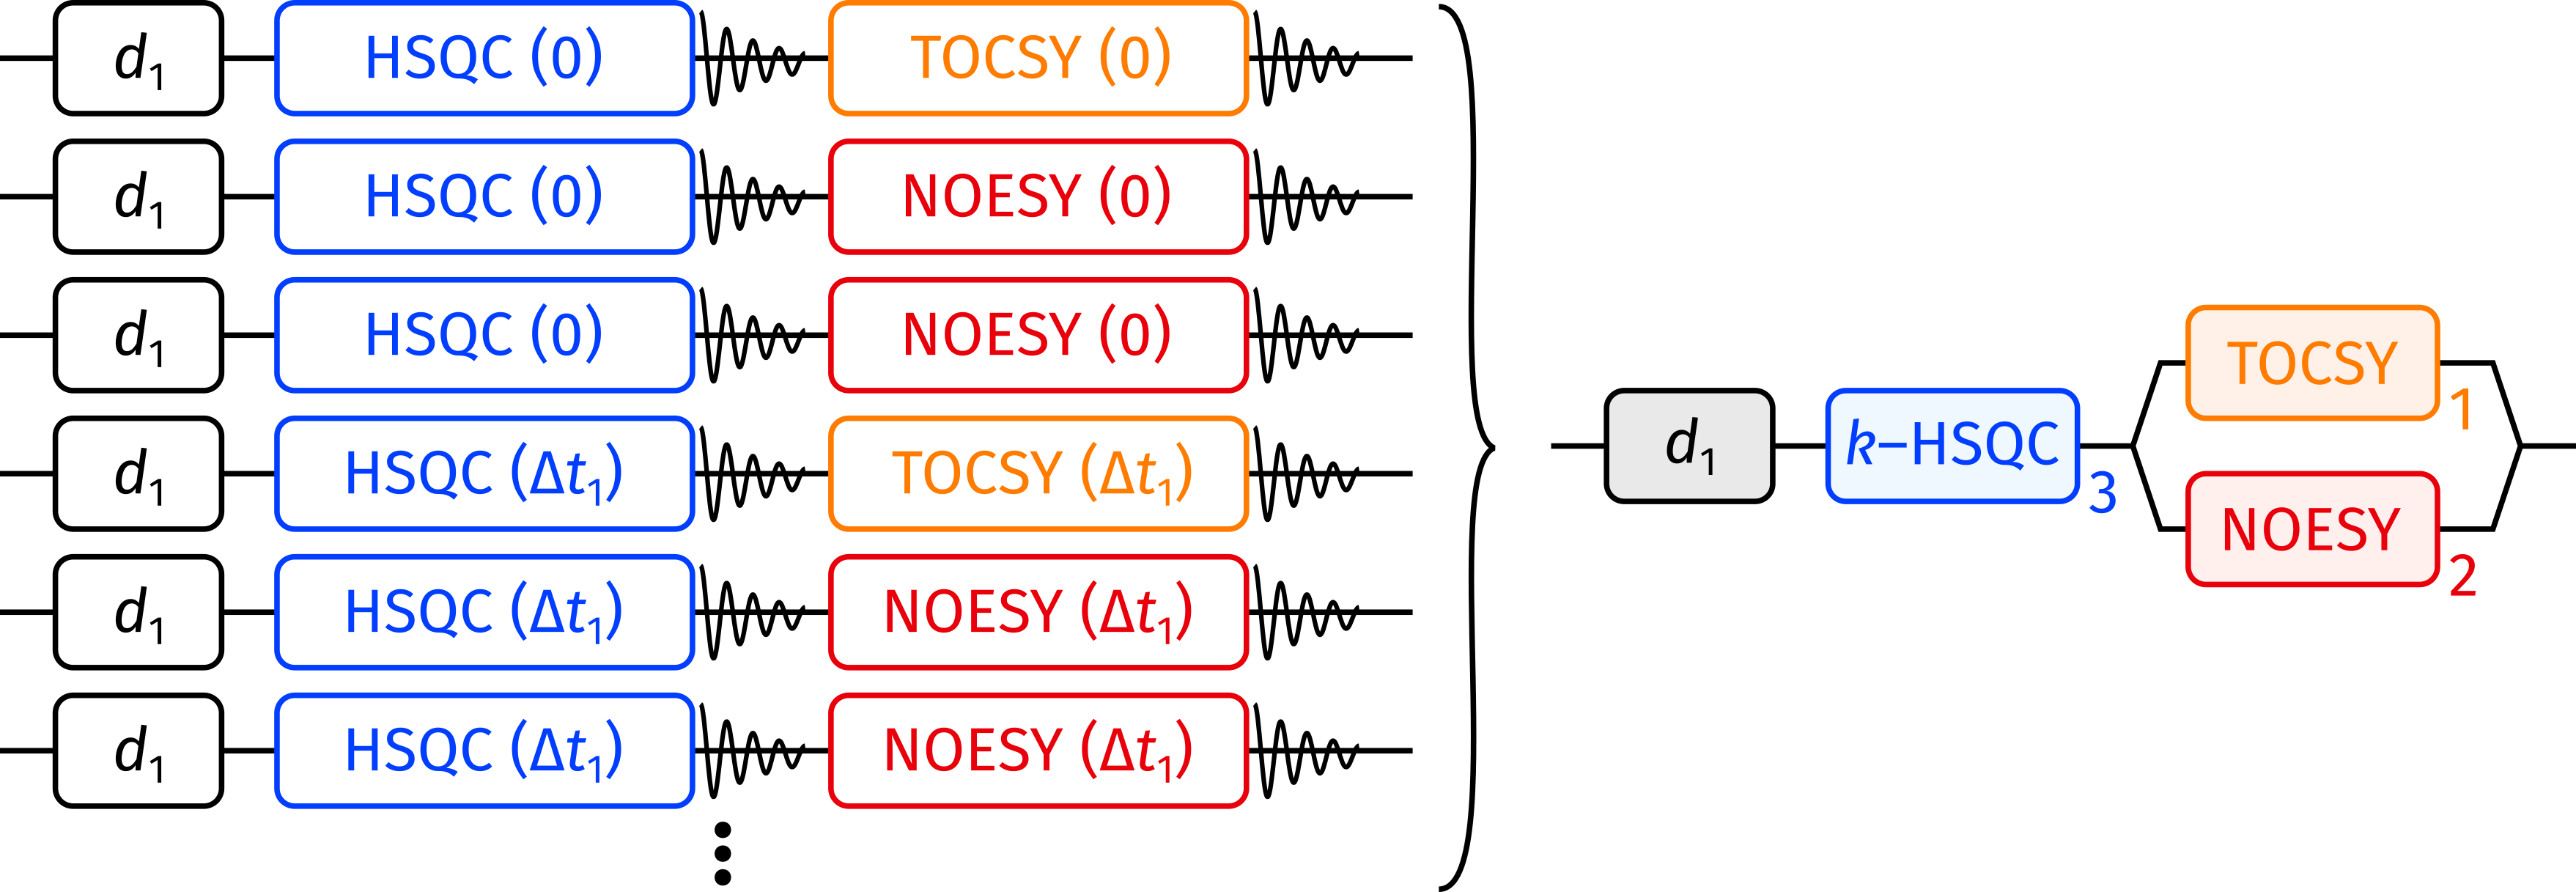
\includegraphics[draft=false]{noah/generalised_example.png}%
    \caption[A basic example of a generalised supersequence]{
        A basic example of a `generalised' NOAH supersequence, where an arbitrary number of supersequences (here three) can be vertically `stacked'.
        For each value of $t_1$, the TOCSY is acquired once, the NOESY twice, and the HSQC three times, as indicated by the subscripts in the condensed representation on the right.
    }
    \label{fig:generalised_example}
\end{figure}

\subsubsection{Pulse sequence implementation}

Unfortunately, GENESIS is not (at present) advanced enough to create pulse programmes generalised supersequences.
Thus, the pulse programmes for this section have been written by hand.
The overall structure of such a pulse programme is shown in \cref{lst:generalised_pp}.
The parameter \texttt{CNST51} corresponds to the number of supersequences being interleaved, i.e., $M$ in the discussion above.
The values of $m_1$ and $m_2$ are encoded as \texttt{CNST52} and \texttt{CNST53}; the latter of these can be automatically calculated.

\begin{mylisting}[!htbp] % lst:generalised_pp {{{1
\begin{tcbminted}{bruker}
"l0     = td1/2"             ; TD1/NBL
"cnst53 = cnst51 - cnst52"   ; automatically calculate m_2 = M - m_1
; ...

1 ze
2 30m
4 50u UNBLKGRAD
  d1 st0

  ; HSQC goes here
  ; ...
  goscnp ph30 cpd2:f2
  50u do:f2

  ; check which module to run
  if "l3 % cnst51 < cnst52"
{
  ; TOCSY goes here
  ; ...
  go=2 ph31
}
  else
{
  ; NOESY goes here
  ; ...
  go=2 ph31
}

  ; move to next 'row' in diagram
  1m iu3
  30m wr #0 if #0 zd

  ; check if M 'rows' have passed
  if "l3 % cnst51 == 0"
{
  1m iu1
  1m igrad EA   ; HSQC echo-antiecho gradients
  ; ...
}

  lo to 4 times l0
end
\end{tcbminted}
    \caption[Structure of pulse programme for generalised supersequences]{
        The overall structure of the pulse programme for the generalised supersequence in \cref{fig:generalised_example}.
    }
    \label{lst:generalised_pp}
\end{mylisting} % }}}1

This structure provides a clear blueprint for how GENESIS can be adapted to produce generalised supersequences.
The only thing which GENESIS needs to detect is how many modules are being interleaved, which determines the number of $m_i$'s.
It should be noted that the `parallel' supersequence of \cref{fig:parallel_noah_overview_kscaled} can be obtained by setting $M = 2$ and $m_1 = m_2 = 1$, and standard linear supersequences simply have $M = m_1 = 1$.
Thus, if generalised supersequences were to be implemented in GENESIS, all other types of supersequences can be obtained `for free'.

A small technical detail in \cref{lst:generalised_pp} is that each \texttt{go=2} statement loops back to the label \texttt{2}, such that the experiment is repeated \texttt{NS} times.
This means that in the left side of \cref{fig:generalised_example}, each row is already acquired a total of \texttt{NS} times, in addition to any repetition which is explicitly shown.
Thus, after summation of the explicitly repeated increments, the HSQC will in fact end up with a total of \texttt{3*NS} scans.
However, the \textit{phase cycle} is only moved forward within the \texttt{NS} loop; each time \texttt{NS} repetitions are completed, the phase cycle is reset to the beginning.
This means that even though each FID in the HSQC is acquired \texttt{3*NS} times, only an \texttt{NS}-step phase cycle is used.
Thus, in order to obtain spectra of the highest possible quality, any common divisors of $M$ and the $m_i$'s should be factorised out and placed into \texttt{NS} instead.


\subsubsection{Examples}

\begin{figure}[!ht]
    \centering
    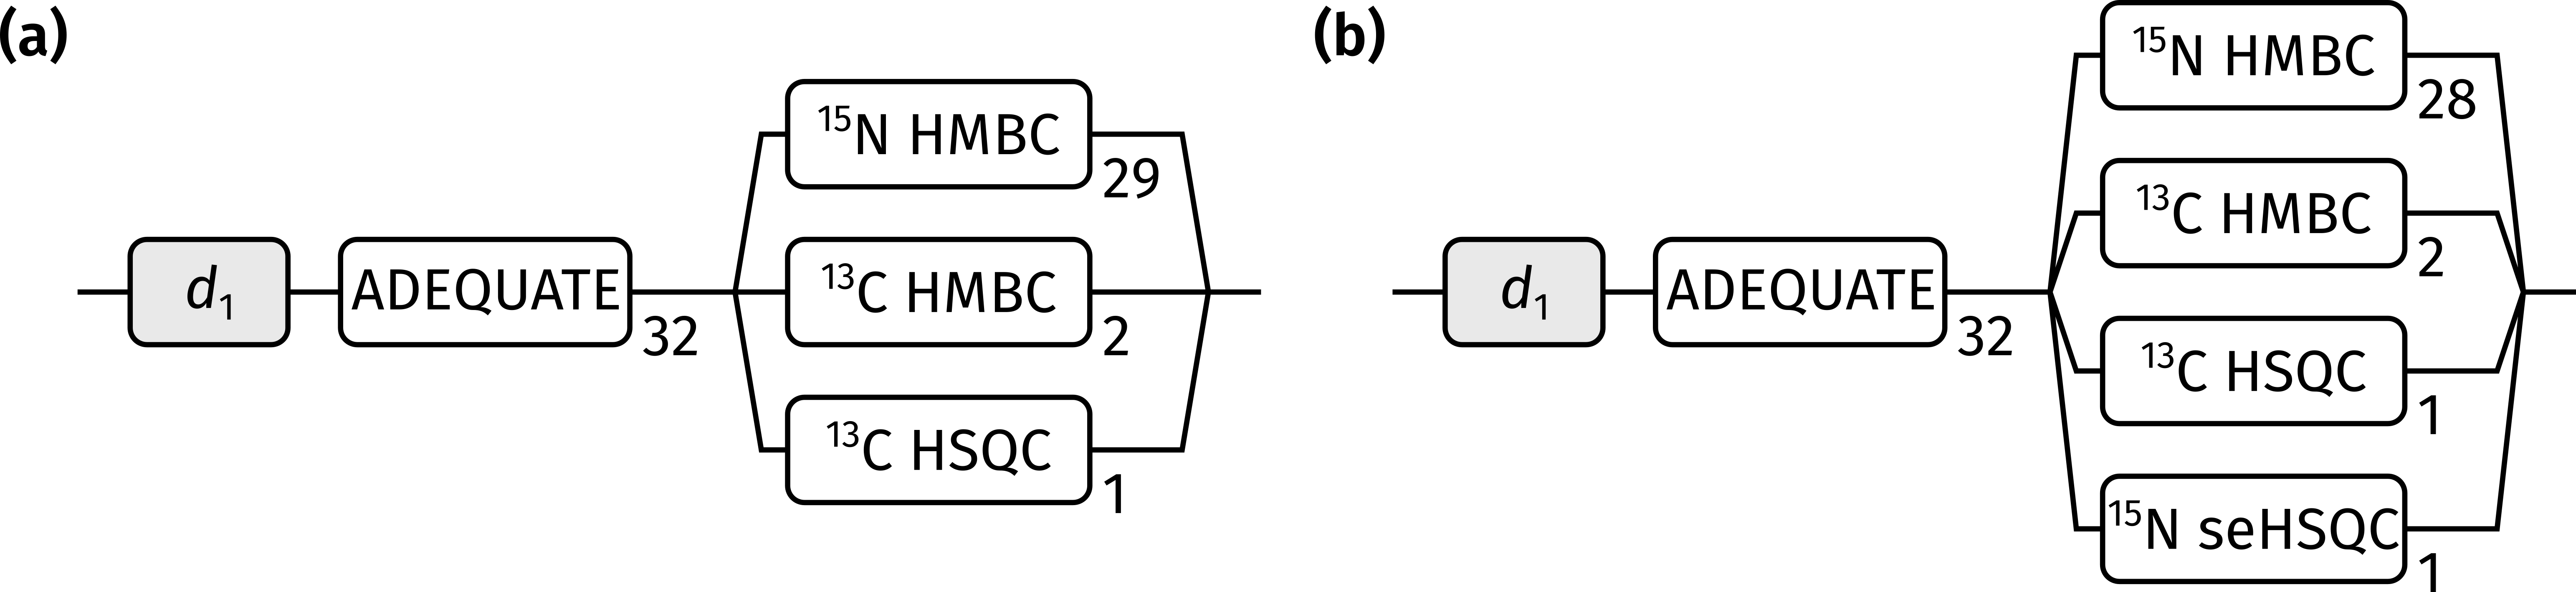
\includegraphics[draft=false]{noah/abbs_pp.png}%
    {\phantomsubcaption\label{fig:abbs_pp_abbs}}%
    {\phantomsubcaption\label{fig:abbs_pp_abbss}}%
    \caption[Examples of generalised supersequences]{
        Two examples of generalised NOAH supersequences.
        \textbf{(\subref*{fig:abbs_pp_abbs})} A \noah{A,Bn,B,S} supersequence.
        \textbf{(\subref*{fig:abbs_pp_abbss})} A \noah{A,Bn,B,S,Spn} supersequence.
    }
    \label{fig:abbs_pp}
\end{figure}

Since generalised supersequences allow the effective number of scans to be individually customised for each module, they offer an avenue for modules with (very) different intrinsic sensitivities to be combined.
On the very-low-sensitivity end are spectra such as ADEQUATE and \nitrogen{} HMBC; compared to these, the HSQC experiments may be considered high-sensitivity.
It should be reiterated that the time savings to be obtained through this combination ($\rho_t$) are still on the order of 2, because only two modules are being horizontally concatenated at a time.


\begin{figure}[!htb]
    \centering
    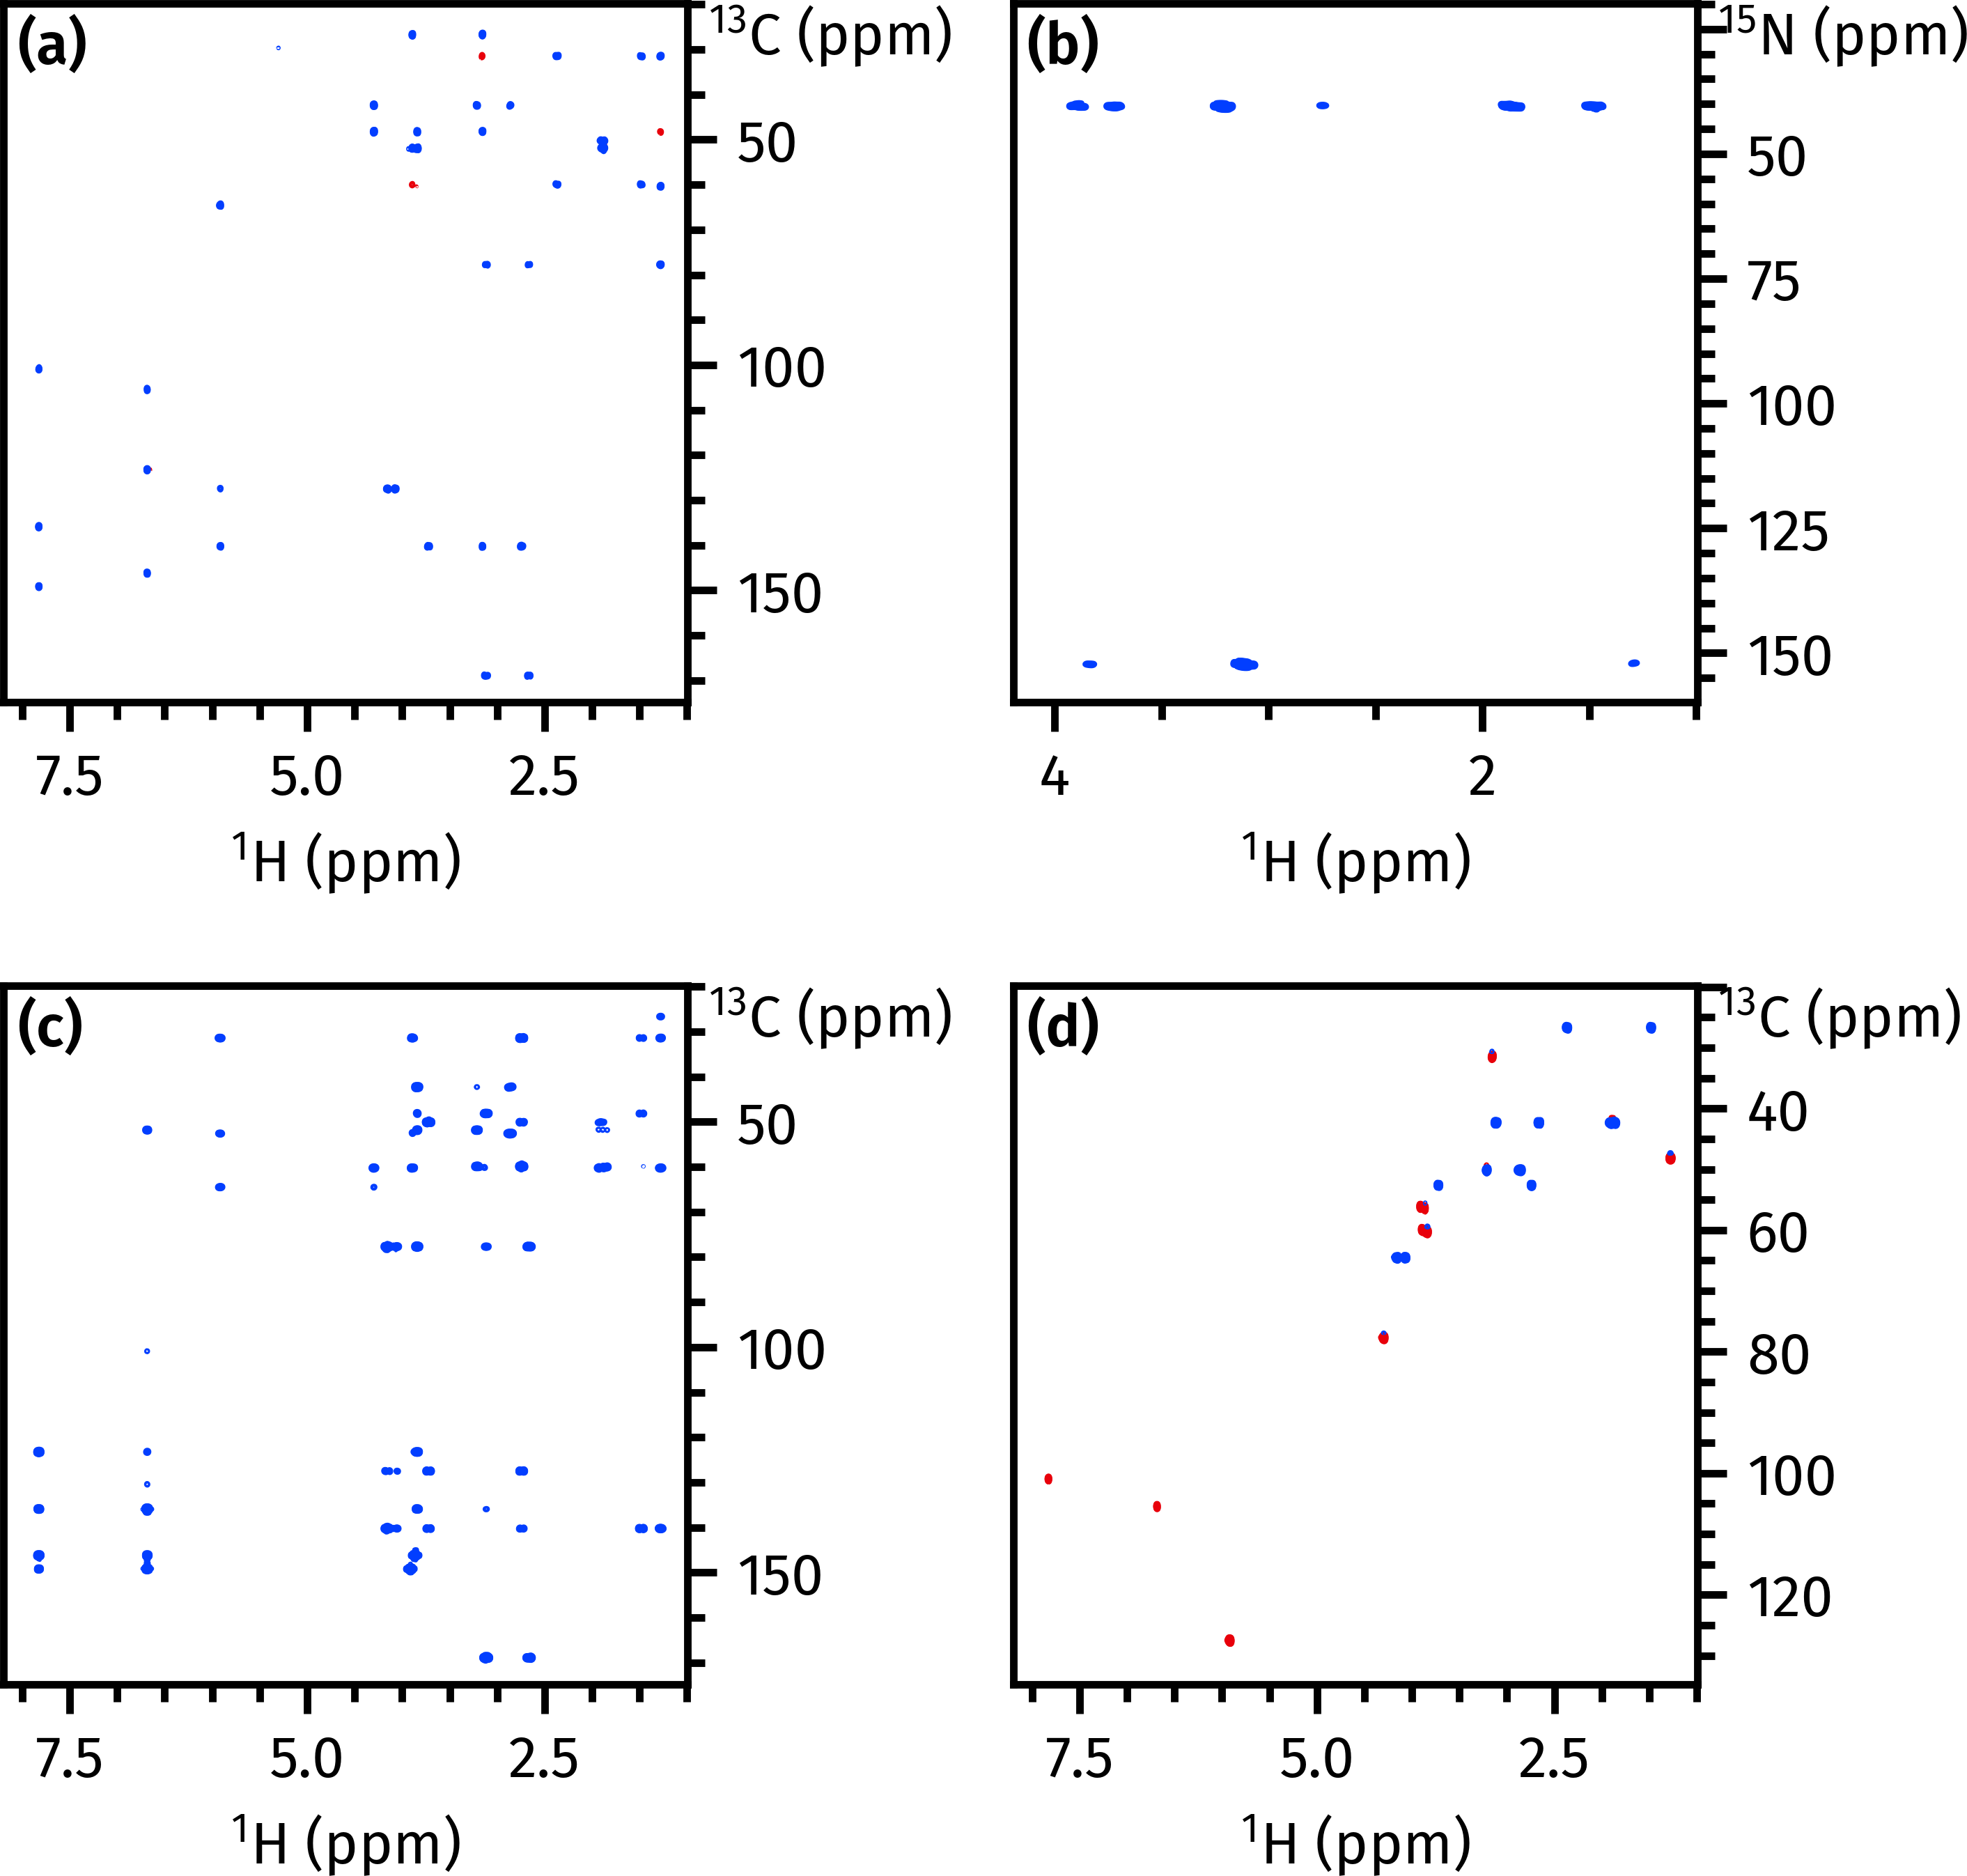
\includegraphics[draft=false]{noah/abbs_spec.png}%
    {\phantomsubcaption\label{fig:abbs_spec_a}}%
    {\phantomsubcaption\label{fig:abbs_spec_bn}}%
    {\phantomsubcaption\label{fig:abbs_spec_b}}%
    {\phantomsubcaption\label{fig:abbs_spec_s}}%
    \caption[Spectra from \noah{A,Bn,B,S} generalised supersequence]{
        Spectra from the \noah{A,Bn,B,S} generalised supersequence (\cref{fig:abbs_pp_abbs}).
        \textbf{(\subref*{fig:abbs_spec_a})} ADEQUATE.
        \textbf{(\subref*{fig:abbs_spec_bn})} \nitrogen{} HMBC, optimised for an $\nJ{NH}$ value of \qty{8}{\Hz}.
        \textbf{(\subref*{fig:abbs_spec_b})} \carbon{} HMBC, optimised for an $\nJ{CH}$ value of \qty{8}{\Hz}.
        \textbf{(\subref*{fig:abbs_spec_s})} \carbon{} HSQC.
        \datacode{7X-220604}
    }
    \label{fig:abbs_spec}
\end{figure}

\begin{figure}[!ht]
    \centering
    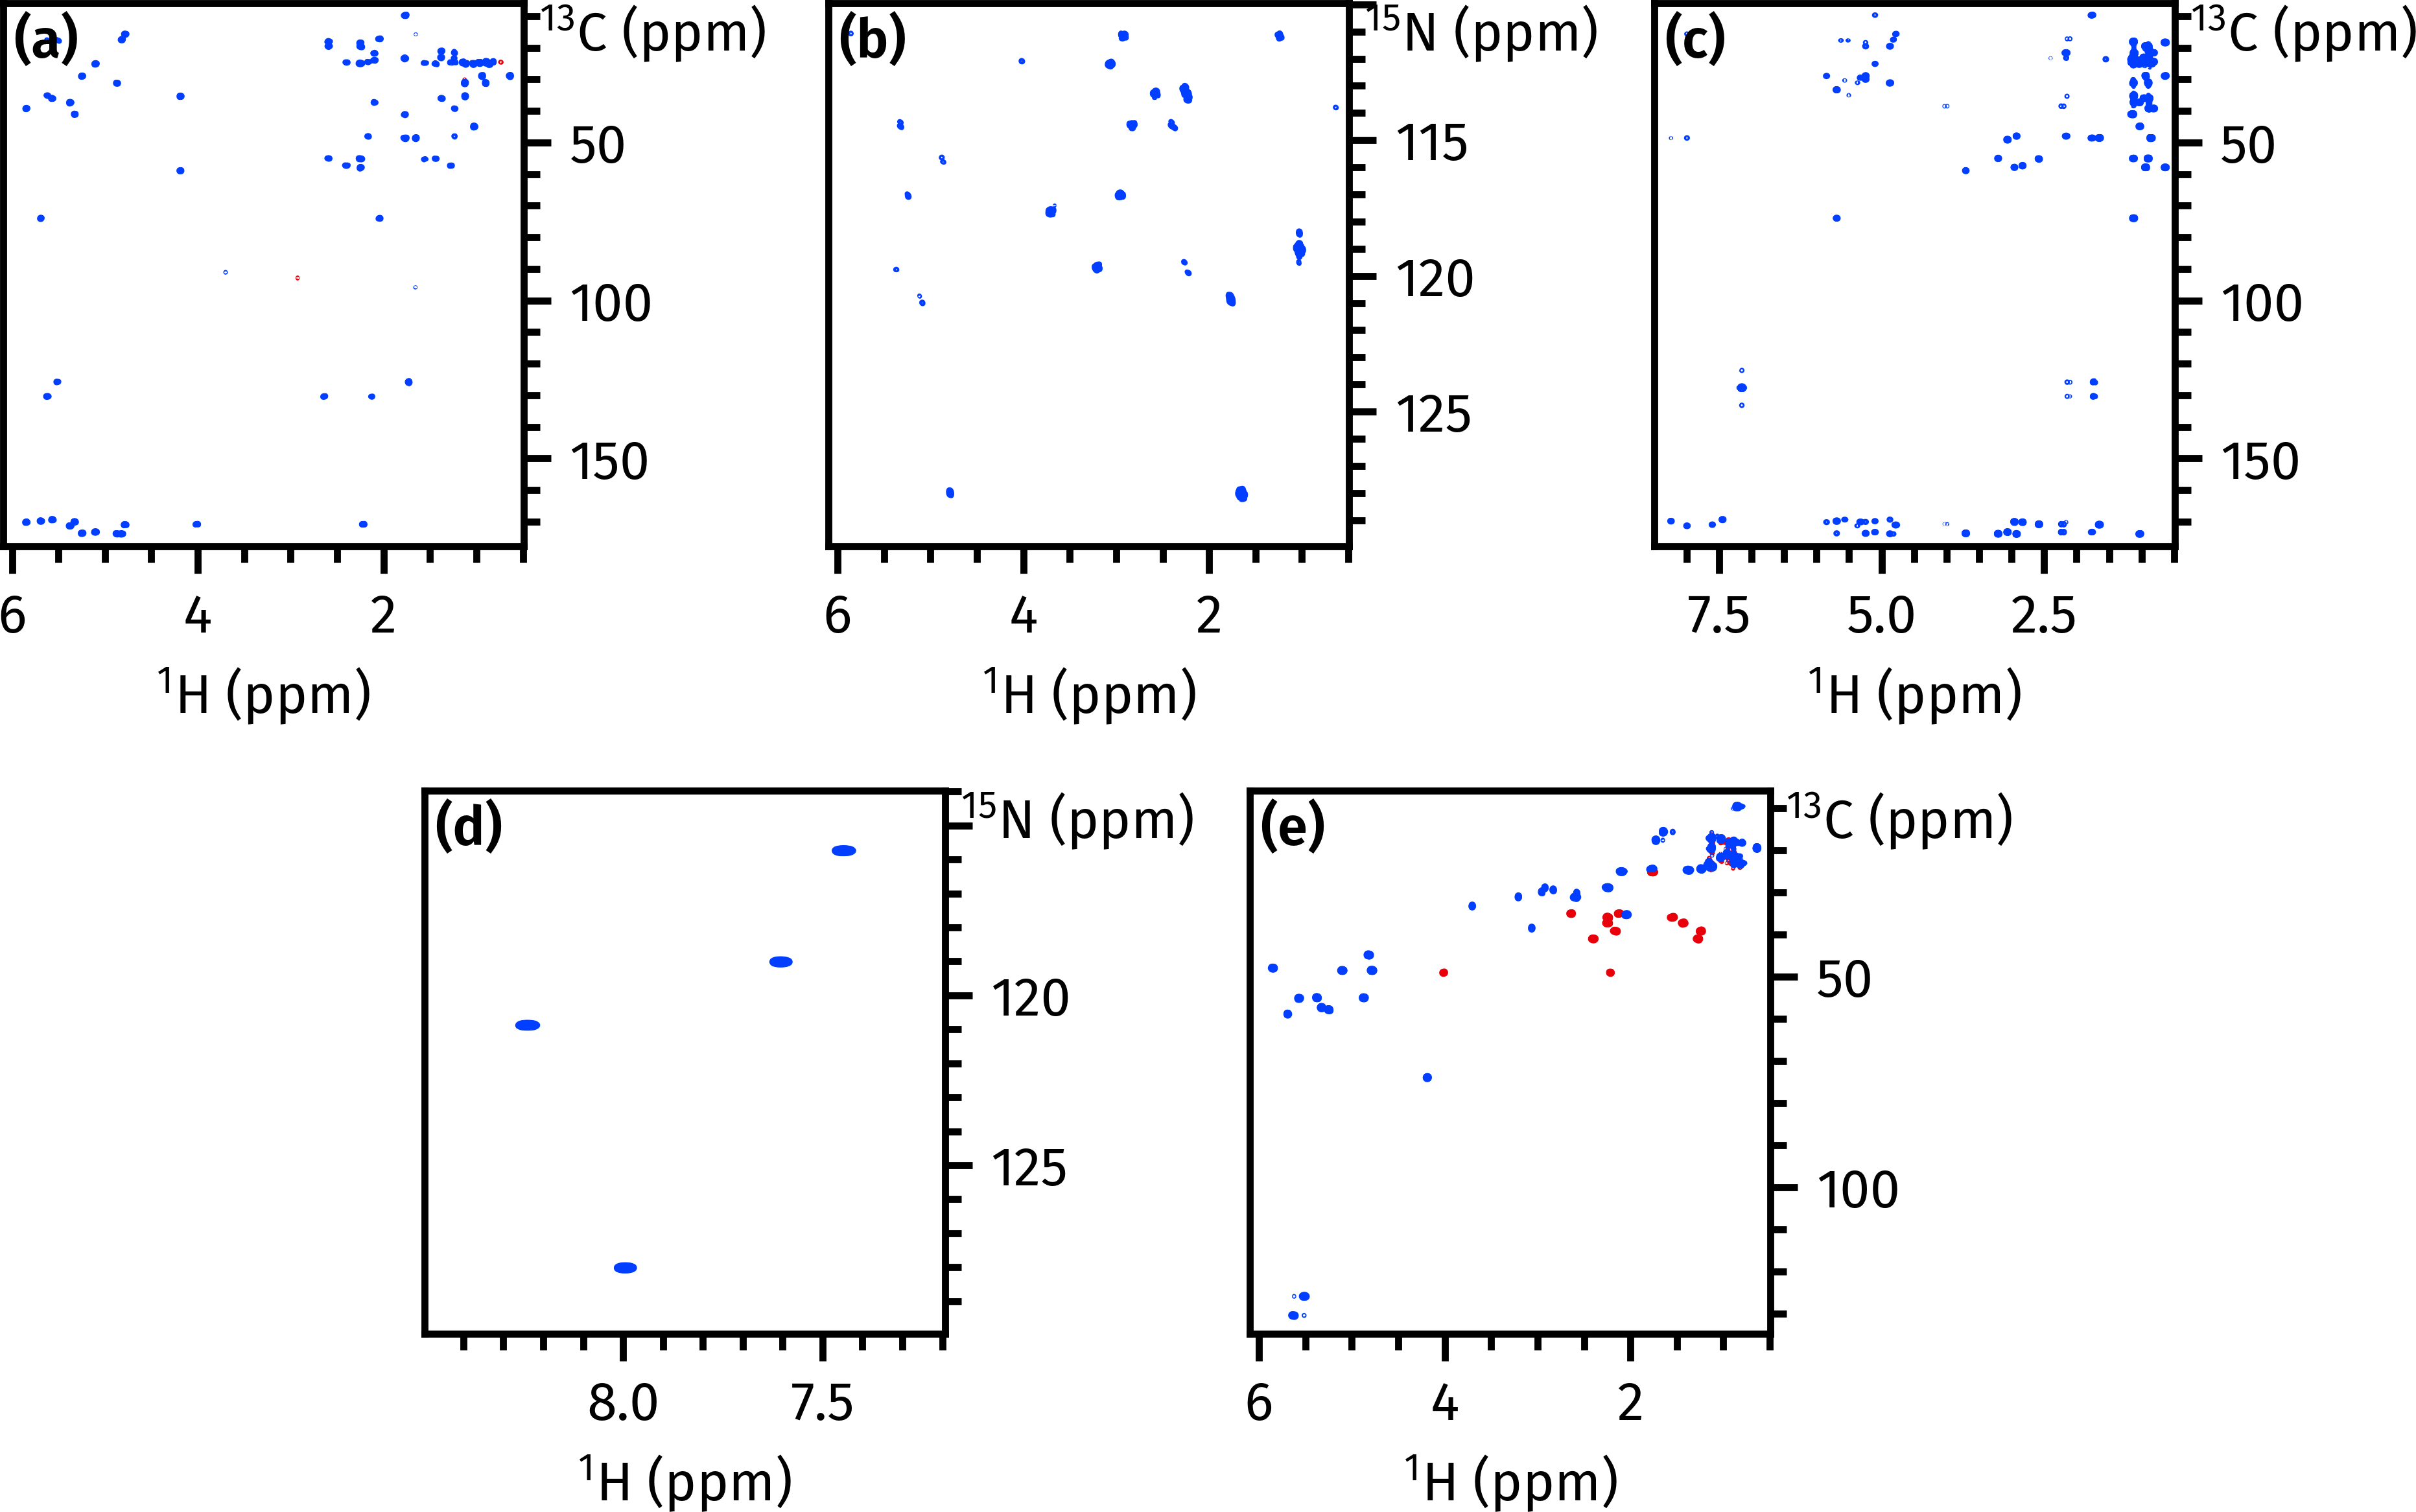
\includegraphics[draft=false]{noah/abbss_spec.png}%
    {\phantomsubcaption\label{fig:abbss_spec_a}}%
    {\phantomsubcaption\label{fig:abbss_spec_bn}}%
    {\phantomsubcaption\label{fig:abbss_spec_b}}%
    {\phantomsubcaption\label{fig:abbss_spec_s}}%
    {\phantomsubcaption\label{fig:abbss_spec_sn}}%
    \caption[Spectra from \noah{A,Bn,B,S,Spn} generalised supersequence]{
        Spectra from the \noah{A,Bn,B,S,Spn} generalised supersequence (\cref{fig:abbs_pp_abbss}).
        \textbf{(\subref*{fig:abbss_spec_a})} ADEQUATE.
        \textbf{(\subref*{fig:abbss_spec_bn})} \nitrogen{} HMBC, optimised for an $\nJ{NH}$ value of \qty{4}{\Hz}.
        \textbf{(\subref*{fig:abbss_spec_b})} \carbon{} HMBC, optimised for an $\nJ{CH}$ value of \qty{8}{\Hz}.
        \textbf{(\subref*{fig:abbss_spec_sn})} \nitrogen{} seHSQC.
        \textbf{(\subref*{fig:abbss_spec_s})} \carbon{} HSQC.
        \datacode{7C-220722}
    }
    \label{fig:abbss_spec}
\end{figure}

\Cref{fig:abbs_pp} shows some examples of such experiments, where the relative numbers of scans are chosen with the aim of balancing the sensitivities of each module.
The ADEQUATE module used here is the ZIP-ADEQUATE experiment shown in \cref{fig:adequate_noah}; this consumes \magn{C} magnetisation and preserves the \magnnot{C} magnetisation required by the \nitrogen{} HMBC, \carbon{} HMBC, and \nitrogen{} seHSQC.
However, the \carbon{} HSQC module draws on the same magnetisation pool; therefore, in order to maximise the intensities in this experiment, a period of isotropic mixing is applied only before the HSQC module in order to effect polarisation transfer from \magnnot{C} spins.
The spectra thus obtained are shown in \cref{fig:abbs_spec,fig:abbss_spec}.

Another additional implementation detail, related to the earlier point about phase cycling, is that on each repetition of the ADEQUATE/\nitrogen{} HMBC increments, the \nitrogen{} HMBC signal (specifically, the first \nitrogen{} \ang{90} pulse) and receiver phases are additionally inverted.
This can be accomplished by adding the corresponding extra phase incrementation instructions just underneath the \texttt{1m iu3} line in \cref{lst:generalised_pp}, and can be thought of as a form of `manual' phase cycling, which is independent of (and complementary to) the usual phase cycle specified in the pulse programme.
The reason for doing this is to suppress artefacts which appear at $F_1 \approx 0$ in the \nitrogen{} HMBC, which stem from the ADEQUATE module (when the \nitrogen{} HMBC is run on its own, these artefacts do not appear).
The exact origin of these artefacts is still unclear,%
\footnote{Their frequencies in $F_1$ are not exactly zero, so there is \textit{some} kind of modulation in the $t_1$ period of the ADEQUATE module, but it is not entirely clear where this is happening. My current best guess is that the offending magnetisation evolves during the constant-time period of the ADEQUATE, where the double-quantum frequencies are reconverted into single-quantum frequencies.}
but their phase is constant; thus, inverting the \nitrogen{} HMBC receiver phase leads to their cancellation.
It should be noted that the issue of phase cycling is not unique to generalised supersequences: indeed, such phase cycling would also be necessary in a standard linear \noah{A,Bn} supersequence.
However, because the degree of built-in phase cycling in a generalised supersequence is lower than the actual number of transients recorded for each module, some of it must be explicitly specified in this way.


\subsubsection{Covariance analysis}

The generalised supersequences shown in \cref{fig:abbs_pp,fig:abbs_spec,fig:abbss_spec} yield very thorough information about heteronuclear connectivity, including one-bond and long-range \proton{}--\carbon{} and \proton{}--\nitrogen{} couplings.
These spectra can be used as inputs for indirect covariance processing\autocite{Zhang2004JACS,Snyder2009JPCA,Jaeger2014ARNMRS} in order to yield `unnatural' (but very informative) double heteronuclear correlation spectra, in which each peak represents a correlation between two dilute heteronuclei (\carbon{} or \nitrogen{}).
Directly recording such spectra through an NMR experiment would require substantially more time, because of the extremely low probability of finding two heteronuclei in the same isotopologue.

Some possible covariance spectra obtained from the data in \cref{fig:abbs_spec,fig:abbss_spec} are shown in \cref{fig:covariance_spec}.
All covariance calculations were performed in Python, according to the formulae:
\begin{equation}
    \label{eq:covariance_unsymmetrical}
    \symbf{C} = \symbf{S}_1\symbf{S}_2^T
\end{equation}
for unsymmetrical indirect covariance (where $\symbf{S}_1$ and $\symbf{S}_2$ are the input spectra and $\symbf{C}$ the covariance spectrum), or
\begin{equation}
    \label{eq:covariance_generalised}
    \symbf{M} = \left[\begin{pmatrix}\symbf{S}_1 \\ \symbf{S}_2\end{pmatrix}
    \begin{pmatrix}\symbf{S}_1 & \symbf{S}_2 \end{pmatrix}\right]^\lambda
\end{equation}
for generalised indirect covariance; the covariance spectrum $\symbf{C}$ can then be obtained as an off-diagonal block of the matrix $\symbf{M}$.
$\lambda$ is a parameter which is chosen in order to balance peak intensity and artefact intensity\autocite{Snyder2009JPCA}.

In \cref{fig:covariance_spec_bruc_cn}, the brucine \nitrogen{} HMBC and \carbon{} HSQC spectra  (\cref{fig:abbs_spec_bn,fig:abbs_spec_s}) are processed using unsymmetrical indirect covariance to yield a \carbon{}--\nitrogen{} correlation spectrum which contains both one- and long-range correlations.\autocite{Martin2007JHC,Martin2007MRC}
The sign of the peaks indicates the multiplicity of the \carbon{} involved, and stems from the use of multiplicity editing in the \carbon{} HSQC spectrum.
Unfortunately, one of the weaknesses of covariance spectra is on show here: there are several artefacts in this spectrum (marked by asterisks), caused by overlap in the \proton{} dimension of both input spectra.

The other three spectra (\cref{fig:covariance_spec_cyclo_caco,fig:covariance_spec_cyclo_cacb_nosymm,fig:covariance_spec_cyclo_cacb_symm}) combine the cyclosporin \carbon{} HSQC and ADEQUATE modules (\cref{fig:abbss_spec_a,fig:abbss_spec_s}) to generate a \carbon{}--\carbon{} one-bond correlation spectrum: essentially, an INADEQUATE spectrum (but with single-quantum frequencies in both dimensions)\autocite{Martin2011MRC,Martin2011MRC2}.
This should in principle be symmetric about the main diagonal.
However, since the HSQC only detects protonated carbons, and the ADEQUATE input spectrum only detects correlations involving at least one protonated carbon.
Thus, correlations between two quaternary carbons do not appear, and correlations between protonated and quaternary carbons only appear once in the spectrum (instead of twice).
This does not a problem in the case of cyclosporin, though, as the only quaternary carbons are those of the carbonyl (\ch{CO}) group, which will still display correlations to the adjacent \ch{C}$\alpha$ carbons.

These \ch{C}$\alpha$--\ch{CO} correlations are shown in \cref{fig:covariance_spec_cyclo_caco}.
There are 11 peaks here, one for each amino acid residue in cyclosporin: again, the sign indicates the \ch{C}$\alpha$ multiplicity (all are \ch{CH} except for the \textit{N}-methylglycine \ch{CH2}).
In \cref{fig:covariance_spec_cyclo_cacb_nosymm,fig:covariance_spec_cyclo_cacb_symm}, the \ch{C}$\alpha$--\ch{C}$\beta$ correlations are shown.
This part of the spectrum has been further subjected to a sign-preserving symmetrisation procedure, where the intensity at each point $p(\Omega_1, \Omega_2)$ is replaced by
\begin{equation}
    \label{eq:covariance_symmetrisation}
    p(\Omega_1, \Omega_2) = \sgn[p(\Omega_1, \Omega_2)] \cdot \min\left\{|p(\Omega_1, \Omega_2)|, |p(\Omega_2, \Omega_1)|\right\}.
\end{equation}
Here, $\sgn{x}$ refers to the sign of $x$, or equivalently $x / |x|$ (for $x \neq 0$).
Since all \ch{C}$\alpha$ and \ch{C}$\beta$ carbons in cyclosporin are protonated, the spectrum is expected to be symmetric; this symmetrisation process therefore helps to remove some of the artefacts which tend to plague the interpretation of covariance spectra.

\begin{figure}[!ht]
    \centering
    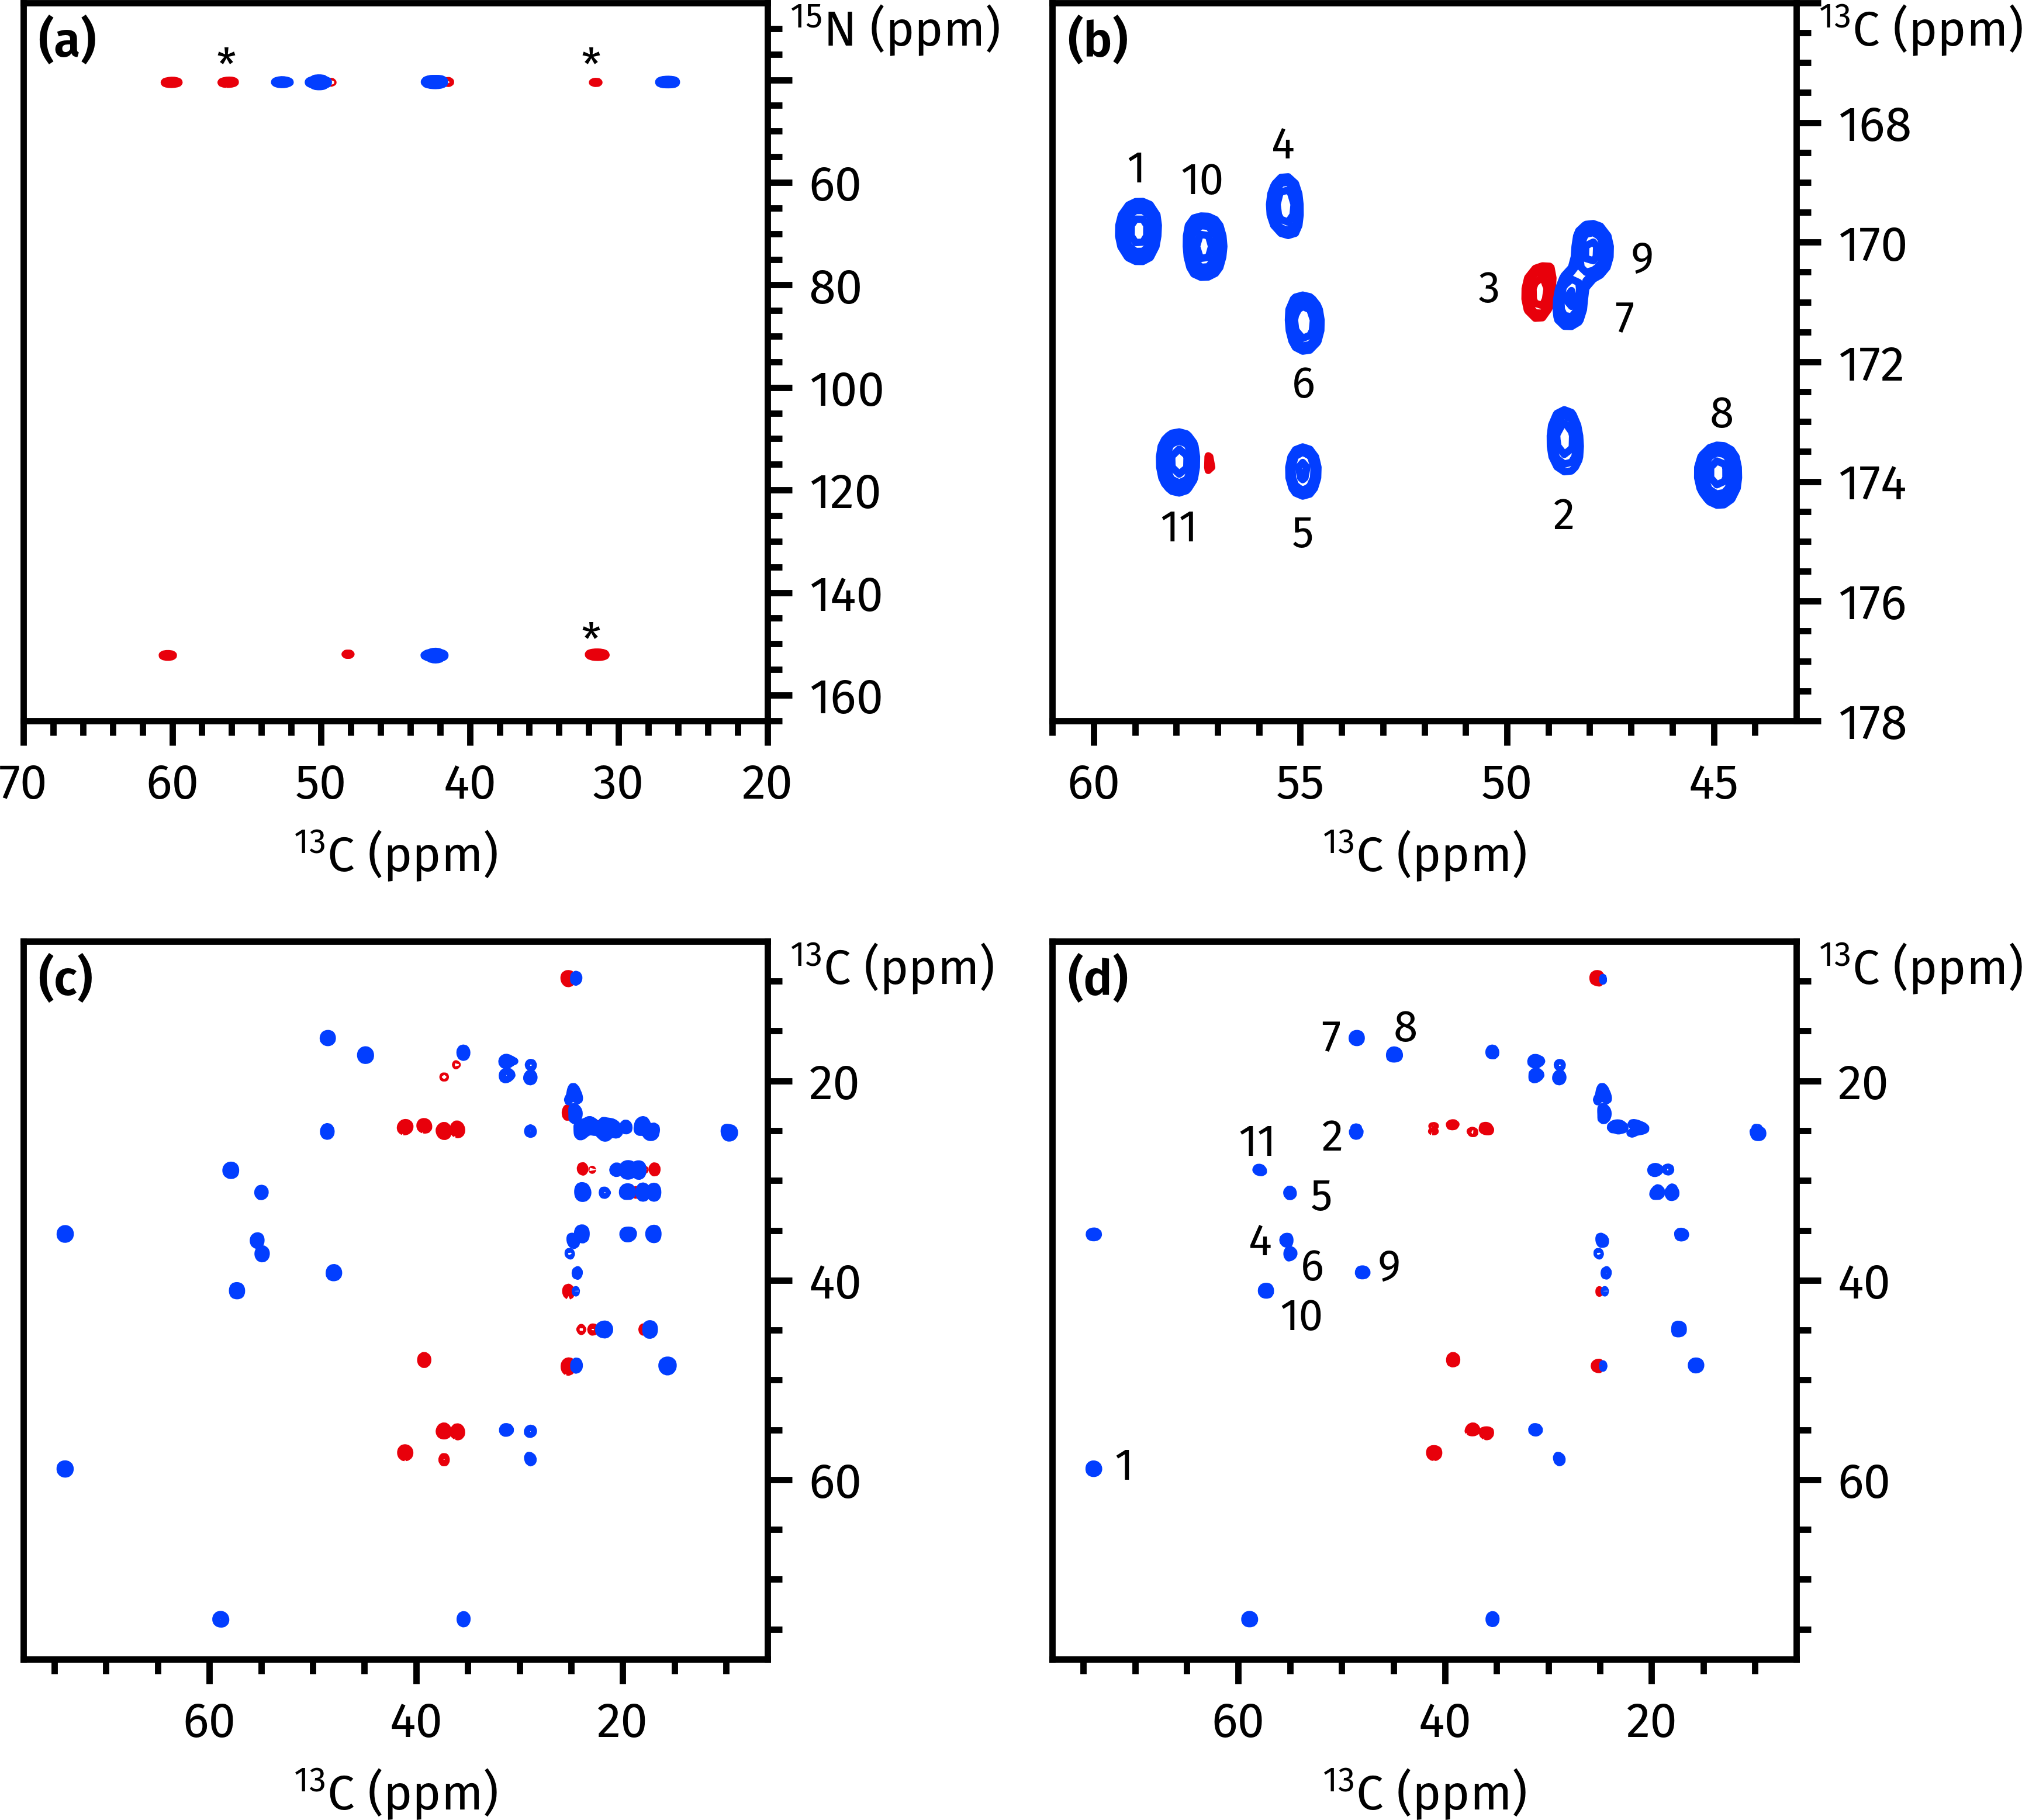
\includegraphics[draft=false]{noah/covariance.png}%
    {\phantomsubcaption\label{fig:covariance_spec_bruc_cn}}%
    {\phantomsubcaption\label{fig:covariance_spec_cyclo_caco}}%
    {\phantomsubcaption\label{fig:covariance_spec_cyclo_cacb_nosymm}}%
    {\phantomsubcaption\label{fig:covariance_spec_cyclo_cacb_symm}}%
    \caption[Examples of covariance spectra obtained from generalised NOAH supersequences]{
        Examples of covariance spectra obtained from generalised NOAH supersequences.
        \textbf{(\subref*{fig:covariance_spec_bruc_cn})} \carbon{}--\nitrogen{} correlation spectrum for brucine.
        Asterisks indicate artefacts arising from peak overlap.
        \textbf{(\subref*{fig:covariance_spec_cyclo_caco})} Inset of the \carbon{}--\carbon{} one-bond correlation spectrum for cyclosporin, obtained by processing the ADEQUATE and \carbon{} HSQC spectra in \cref{fig:abbss_spec_a,fig:abbss_spec_s} using generalised indirect covariance ($\lambda = 0.5$).
        The region shown here contains correlations between \ch{CO} and \ch{C}$\alpha$ carbons.
        \textbf{(\subref*{fig:covariance_spec_cyclo_cacb_nosymm})--(\subref*{fig:covariance_spec_cyclo_cacb_symm})} A different inset from the same \carbon{}--\carbon{} correlation spectrum as in (\subref*{fig:covariance_spec_cyclo_caco}), but this time showing correlations in the alkyl region.
        The spectrum in (\subref*{fig:covariance_spec_cyclo_cacb_symm}) has been further subject to a sign-preserving symmetrisation process.
        The \ch{CO}--\ch{C}$\alpha$ and \ch{C}$\alpha$--\ch{C}$\beta$ correlations for all residues are labelled in (\subref*{fig:covariance_spec_cyclo_caco}) and (\subref*{fig:covariance_spec_cyclo_cacb_symm}) (following the numbering in \todo{REF}).
    }
    \label{fig:covariance_spec}
\end{figure}
